\documentclass{report}
\usepackage[utf8]{inputenc}
\usepackage{fancyhdr}
\usepackage{array}
\usepackage{dirtytalk}
\usepackage{graphicx}
\usepackage{caption}
\usepackage{subcaption}
\usepackage{version}
\usepackage{float}

\pagestyle{fancy}
\fancyhead{}
\renewcommand{\chaptername}{Section}
\renewcommand{\chaptermark}[1]{
\markboth{\chaptername
\ \thechapter . \ #1}{}}
\lhead{\slshape\leftmark}
\lfoot{F. Comolli, F. Corda}
\rfoot{DD v1.1}
\renewcommand{\headrulewidth}{0.4pt}
\renewcommand{\footrulewidth}{0.4pt}

\author{Federico Comolli
        \and
        Francesco Corda}
\date{October 2018}


\usepackage{graphicx}
\usepackage[nottoc,numbib]{tocbibind}
\renewcommand\bibname{References}

\usepackage{hyperref}
\hypersetup{
    colorlinks,
    citecolor=black,
    filecolor=black,
    linkcolor=black,
    urlcolor=black
}

\usepackage{enumitem}

\usepackage[dvipsnames]{xcolor}
\usepackage{listings}

\usepackage{spreadtab}
\usepackage{fp}
\usepackage{xstring}

\usepackage{pdflscape}
\usepackage{pdfpages}

\begin{document}

\begin{titlepage}
	\centering
	
\includegraphics[width=150pt]{images/polimi_logo}\par\vspace{1cm}
	{\scshape\LARGE
		Politecnico di Milano\par}
	\vspace{1cm}
	{\scshape\Large
		Software Engineering 2 Project\\
		a.y. 2018-19\par}
	\vspace{1.5cm}
	{\huge\bfseries
		Data4Help, AutomatedSOS\\\par}
	{\Large\bfseries
		Design Document\par}
	Version 1.1\par
	\vspace{2cm}
	{\Large
		Comolli Federico, 920258\\
	    Corda Francesco, 920912\par}
	\vfill
	Referent Professor: Di Nitto Elisabetta\par
	\vfill
	{\large\today\par}
\end{titlepage}


\renewcommand{\contentsname}{Table of Contents}
\tableofcontents

\chapter{Introduction}
\section{Purpose}
TrackMe is a company that wants to create a software-based system that allow third parties to monitor the location and health status of individuals. 
\par This service, which from now on will be referred to as Data4Help, supports the registration of individuals who, by registering, agree to the collection of their data. Data acquisition can occur through smart watches or similar electronic devices.
\par Third parties can request access to the data of some specific individuals of which they know a form of identification (such as the SSN or the Fiscal Code). In this case, TrackMe forwards the request to the user who can accept or refuse it.
\par Another service offered to third parties by Data4Help is to access to anonymous data of classes of individuals, grouped by different criteria (for example geographical area, age, sex, etc.). Anonymity is a crucial value for TrackMe, so it approves these requests only if third parties cannot go back to users' identity; for this reason requests referred to groups composed by less than 1000 individuals will be denied.
\par After a request has been accepted, third parties can subscribe to the reception of updated data as soon as they are produced.
\par Moreover, in order to exploit the features offered by Data4Help, TrackMe wants to develop a customized SOS service to elderly people. This system, called AutomatedSOS, uses the data collected by Data4Help to monitor the health status of the subscribed customers. Through the real time screening the system is able to react to the variation of the parameters by sending an ambulance to the location of the customer in case of emergency.

\pagebreak
\subsection{Goals}

Data4Help:  
\begin{enumerate} [label={[G\arabic*]}]
    \item Allow a visitor to become registered user after providing credentials.
    \item Monitor the location of users through electronic devices.
    \item Monitor the health status of users through electronic devices.
    \item Allow a user to accept or refuse a request to access to personal data.
    \item Allow third parties to register to the system.
    \item Allow third parties to request an access to users' data.
    \begin{enumerate} [label*={.\arabic*}]
        \item [{[G6.1]}] Allow third parties to request access to data of some specific individuals by providing SSN or Fiscal Code.
        \item [{[G6.2]}] Allow third parties to request access to anonymized data of group of people.
    \end{enumerate}
    \item Accept request for data of group of people only if the system can guarantee the anonymity of the people.
    \item Allow third parties to subscribe to new data and to receive them as soon as they are produced.
\end{enumerate}  
\noindent
AutomatedSOS:
\begin{enumerate} [resume, label={[G\arabic*]}]
    \item Allow a visitor to become registered user after providing credentials.
    \item Monitor the location of users through electronic devices.
    \item Monitor the health status of users through electronic devices.
    \item Send to the location of the customer very quickly an ambulance when such parameters are below certain thresholds. 
\end{enumerate}

\section{Scope}
\subsection{Analysis of the phenomena}
Data4Help application can be used after the registration through the interface on the electronic devices.
People who are for different reasons interested in services have to provide their name, surname, gender, birth date, SSN or Fiscal Code.
\par Users of Data4Help have to wear some kind of electronic devices that record information about their position and their health status.
Data4Help is an application-to-be that is projected to be installed on different wearable electronic devices (smart-watches, smart-bands, etc.) and eventually can interact with other health tools such as heart rate bands, smart scales or similar.
\par To identify the health status, Data4Help search for different parameters provided by sensors on smart-watches or health tools such as heart rate, skin temperature, blood glucose level, weight, etc.
Also, Data4Help acquires the position of its users through GPS technology.
\newline Data acquired by Data4Help may be matter of interest for third parties that can make a request using the functionality provided by the application. If a request is referred to a single user it's necessary to provide his/her SSN or Fiscal Code. In addition it's possible to request data referred to group of people (associated by age, gender, location, etc.). Data4Help has to accept or decline these requests using a defined privacy criteria.
\par Users who receive a request for their personal information can accept or decline it using the provided functionality.
\newline Data4Help offers the possibility to subscribe to data in order to receive the updated ones as soon they are produced.
\par Furthermore, TrackMe wants to build a new application on top of Data4Help, with the purpose of exploiting its functionality to provide an emergency service.
As for Data4Help, registration is necessary to use AutomatedSOS.
\newline AutomatedSOS analyzes real-time data provided by Data4Help technology.
If the software detects an anomaly in the parameters it notifies an emergency to the Operations Center of the National Health Service within 5 seconds. 
From now on the National Health Service is responsible for the first aid and it manages the request accordingly to its own protocol.
The intervention is carried on determining the emergency level and sending an ambulance to the location of the user.

\subsection{Stakeholders}
In this paragraph we analyze all the entities involved in the project of Data4Help and AutomatedSOS.
\par TrackMe is the main stakeholder of the project being that one who commissioned the project and will pay for it.
The core of the two applications are data provided by users that wants to monitor their health status.
Of course, this amount of data is a source of interest for third parties that wants to access it.
\par The National Health Service plays a fundamental role in the realization of AutomatedSOS taking care of the emergency intervention notified by the software-to-be.

\section{Definitions, Acronyms, Abbreviations}
\subsection{Definitions}
\begin{itemize}
    \item Users: people who use the services provided by TrackMe.
    \item Third Parties: entity that are interested to data provided by TrackMe.
    \item National Health Service: the national institution that provides health care to citizens.
    \item Social Security Number: a nine-digit-number that identifies uniquely a citizen.
    \item Fiscal Code: synonym to Social Security Number for Italian people.
    \item Credentials: user name, password, SSN or Fiscal Code.
    \item Anomaly: when the parameters are below a defined threshold. 
    \item Emergency: it occurs when an anomaly is detected.
    \item System: defines the overall set of software components that implement the required functionalities.
\end{itemize}

\subsection{Acronyms}
\begin{itemize}
    \item RASD: Requirements Analysis and Specification Document. 
    \item SSN: Social Security Number.
    \item GPS: Global Position System.
    \item API: Application Programming Interface.
    \item NHS: National Health Service.
\end{itemize}

\subsection{Abbreviation}
\begin{itemize}
    \item {[Gn]}: n-th goal
    \item {[Rn]}: n-th functional requirement
    \item {[Dn]}: n-th domain assumption
\end{itemize}

\section{Revision history}
Version 1.0 delivered on date 11/11/2018.

\section{Reference Documents}
\begin{itemize}
    \item Specification Document: "Mandatory Project Assignment AY 2018-19". 
    \item \href{https://ieeexplore.ieee.org/document/6146379} {29148-2011 - ISO/IEC/IEEE International Standard - Systems and software engineering -- Life cycle processes --Requirements engineering}
\end{itemize}

\section{Document Structure} %bozza di esempio, da riscrivere
\begin{enumerate} [label={Section \arabic*}]
    \item gives an introduction to the problem and describes the purpose of the applications Data4Help and Automated SOS and states their goals. The scope of the two applications is defined.
    \item presents the overall description of the project. The product perspective includes details on the shared phenomena and the domain models. The class diagram describes the domain model used,and the state diagram analyzes the process of arranging a meeting and reaching it in time. Here the majority of functions of the system are more precisely specified, with respect to the already mentioned goals of the system. In the user characteristics section the types of actors that can use the application are described.
    \item contains the external interface requirements, including: user interfaces, hardware interfaces, software interfaces and communication interfaces. Few scenarios describing specific situations are listed here. Furthermore, the functional requirements are defined by using use case and sequence diagram.
    The non-functional requirements are defined through performance requirements, design constraints and software system attributes.
    \item includes the alloy model and the discussion of its purpose. Also, a world generated by it is shown.
    \item shows the effort spent by each group member while working on this project.
    \item includes the reference documents.
\end{enumerate}

\chapter{Architectural Design}
\section{Overview}
This chapter presents a general overview of the system architecture.
The description will concentrate on the logical and physical components that
we choose to build our system. \\
We will start by illustrating the \textit{High Level components} of the system and their interactions. \\
Then, the section \textit{Components view} will focus on describing the single components and their interfaces. \\
The \textit{Deployment view} will provide the strategy we adopted to deploy the system, highlighting the load division between different tiers of the system. \\
In the \textit{Runtime view} we will illustrate different examples of interaction between the components with the use of Sequence Diagrams. \\
The \textit{Component interfaces} contains a description of the interfaces provided by the logical components. \\
The chapter will end with a selection of \textit{Architectural styles and patterns} and \textit{Other design decisions} chosen while composing the application.
\clearpage
\section{High Level Components and their interactions}
The following image illustrates the general architecture on which the system will be based on. Every component can be associated with one of three logical tier: Data, Application, Presentation. \\
This is a standard and well accepted architecture, that will promote the independence between logically separated components. \\
During the design of the application, our focuses are the one illustrated in the RASD document: maintainability, security, reliability and availability. \\
Given the nature of the two applications, a robust design of the Data tier is fundamental for the success of the project. \\
All the information related to the system will be stored in multiple databases. These will be protected from external attacks by a firewall and will be regularly subjected to back-up procedures. \\
The Application tier contains the logic that controls the core services of Data4Help and AutomatedSOS. The applications will be installed on different servers, located in a demilitarized zone. \\
To conclude the general description, the Presentation tier contains the system interface to the external world. The applications will be accessible both by mobile applications and web browsers. \\
Users accessing the applications via internet browsers will interact with a web server that will provide the web interface. The mobile applications instead will communicate directly with the application server. \\

\begin{figure}[ht]
    \centering
    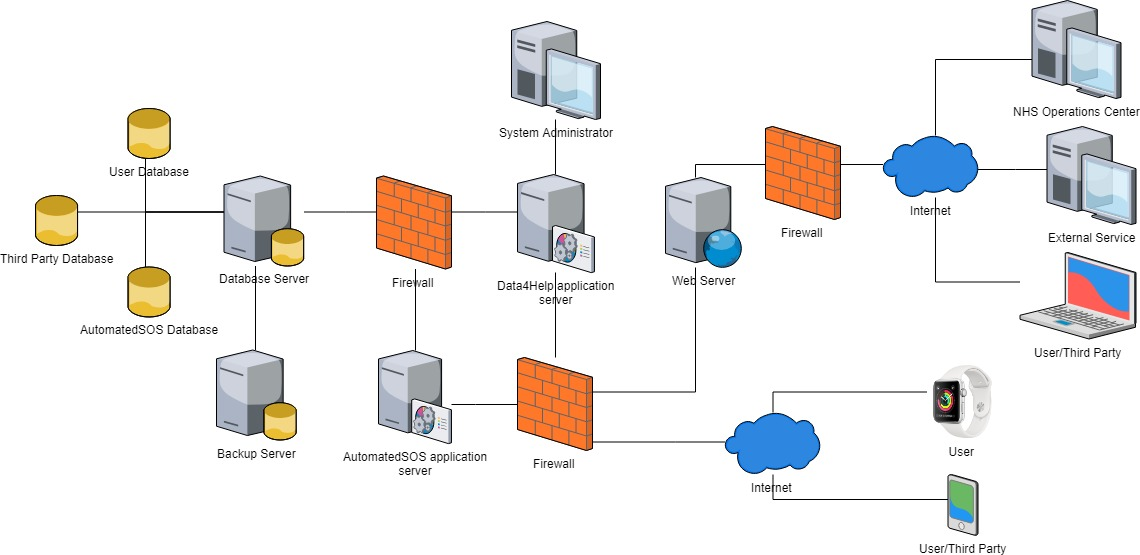
\includegraphics[width=300pt]{images/Overview.jpg}
    \caption{Overview.}
\end{figure}

\clearpage
The UML diagram below describes instead the main logical components that form the system and the connections between them.
Every component enclose a specific group of services offered by the system and is not intended as a node of the physical architecture. \\
Even if this is a very high-level representation of the system it's possible to identify a general subdivision in client-related services, back-end logic and data management components. \\
It is also worth noting relazione tra Automated e Data4help...\\
A more detailed description of each component will be given in the next section. \\

\begin{figure}[ht]
    \centering
    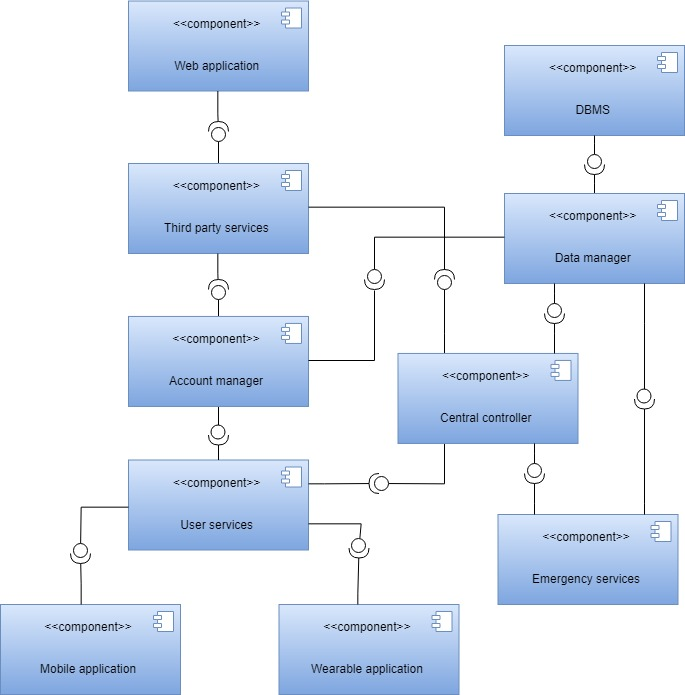
\includegraphics[width=300pt]{images/High-Level_Components.jpg}
    \caption{High Level Components.}
\end{figure}
\clearpage

\hypertarget{CV}{\section{Component	View}}
\begin{figure}[ht]
    \centering
    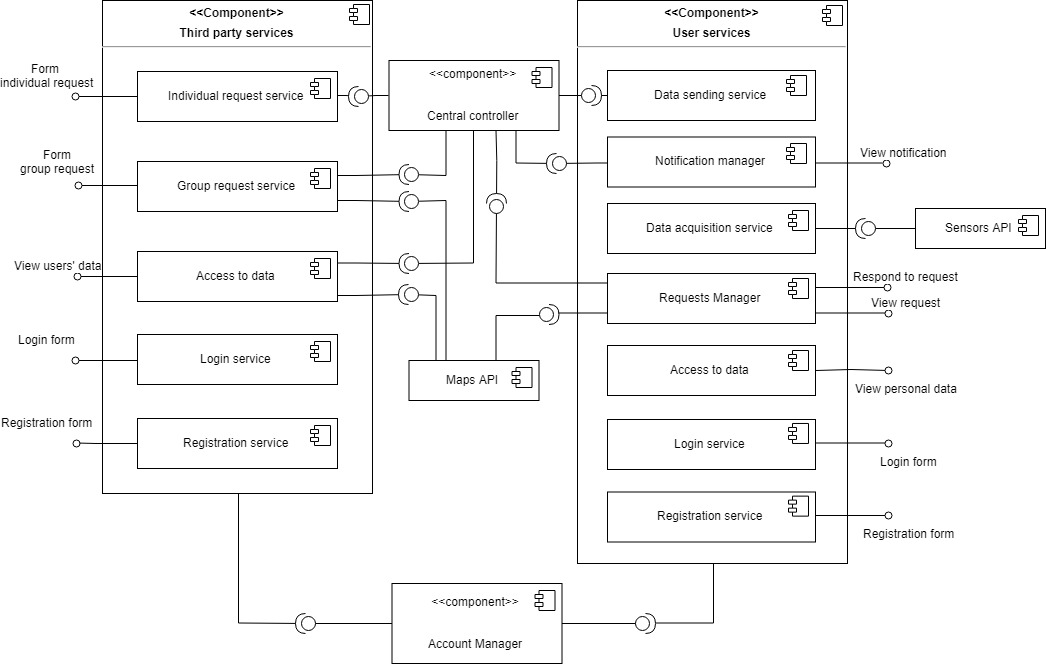
\includegraphics[width=345pt]{images/CompView/Component_view1.jpg}
    \caption{High Level Components.}
\end{figure}
The image above contains an expanded version of the two components User Services and Third Party Services.
We chose to show these components together because of their similarities and common interactions.
These components are responsible to connect the client application with the internal logic.
\textit{Third Party services} provide an interface for every functionality offered to the presentation tier:
\begin{itemize}
    \item \textbf{Individual request service}: module that receives individual requests from a third party \item \textbf{Group request service}: module that receives group requests from a third party
    \item \textbf{Access to data}: provide the access and download of users' data
    \item \textbf{Login Service}: lets the third party sign in to the application
    \item \textbf{Login Service}: lets the third party sign up to the application
\end{itemize}
\textit{User Party services} its the counterpart component for monitored users:
\begin{itemize}
    \item \textbf{Data sending service}: it's the module responsible for sending the user's collected data to Data4Help back-end
    \item \textbf{Notification Manager}: sends notifications to the user
    \item \textbf{Data Acquisition service}: the module that connects with the sensors API to collect the health data and the positions
    \item \textbf{Requests Manager}: module that shows incoming requests to the user and receives their reply  
    \item \textbf{Access to data}: lets the users access and download their data
    \item \textbf{Login Service}: lets the user sign in to the application
    \item \textbf{Login Service}: lets the user sign up to the application
\end{itemize}
Both these components also connects to the Central Controller and the Account Manager modules.

\clearpage

\begin{figure}[ht]
    \centering
    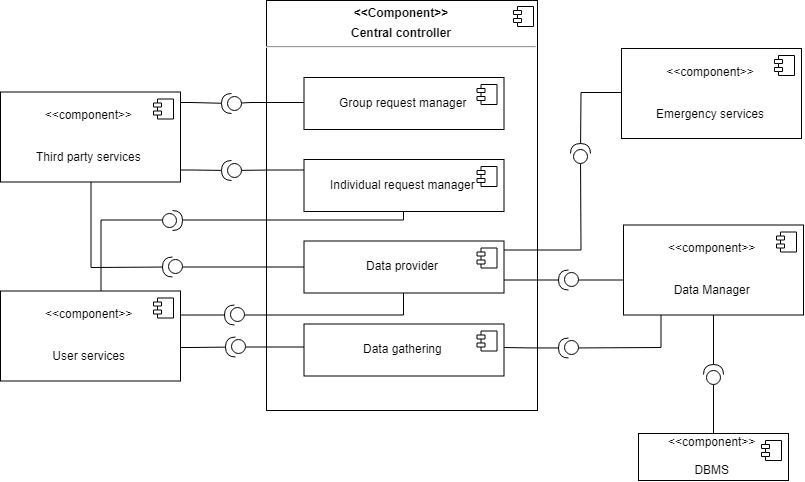
\includegraphics[width=300pt]{images/CompView/Component_view2.jpg}
    \caption{High Level Components.}
\end{figure}
The Central Controller is the core of the system, it's modules manage the acquisition, storing and exchange of data between users and third parties:
\begin{itemize}
    \item \textbf{Group request manager}: this module contains the logic concerning group requests. After receiving a request from a third party, it checks that the privacy condition is respected and authorize or forbid the access to data 
    \item \textbf{Individual request manager}: this module receives the individual requests and forward them to the corresponding user. After receiving the response from the recipient authorize or forbid the access to data
    \item \textbf{Data provider}: service that provides users' data to authorized applicants
    \item \textbf{Data gathering}: module that receives users' data and stores them by using the Data Manager component 
\end{itemize}
\clearpage
\hypertarget{ES}{}
\begin{figure}[ht]
    \centering
    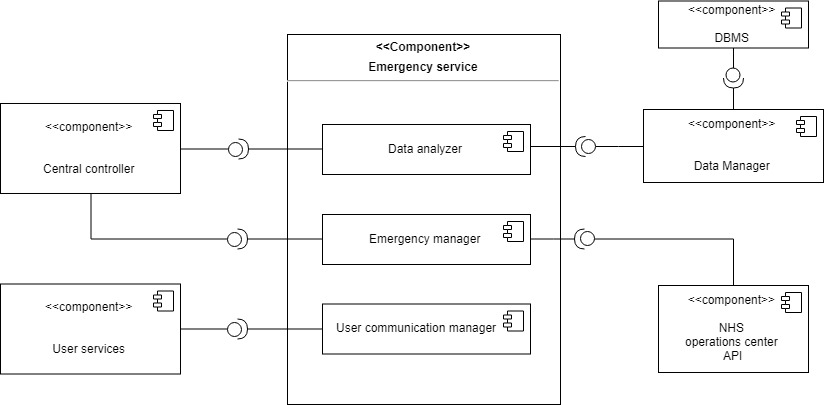
\includegraphics[width=300pt]{images/CompView/Component_view3.jpg}
    \caption{High Level Components.}
\end{figure}
The Emergency Service is the component that manages the logic behind AutomatedSOS. 
One of the...
Since this application is built on top of Data4Help, the emergency service is conceived as a stand-alone module inside the back-end logic of the system.
The two systems share the same Account Manager, so every user that registers to AutomatedSOS is also a Data4Help user. 
FINIRE

\begin{itemize}
    \item \textbf{Data analyzer}: connects with the central controller to acquire users' data and analyzes them in real time. This module also connects with the Data Manager to obtain the parameters thresholds.
    \item \textbf{Emergency Manager}: if the data analyzer detects an anomaly, it alerts the Emergency Manager. This module creates an emergency message containing the user personal credentials, its current position and most recent health parameters. It then sends this message to the NHS.
    \item \textbf{User Communication manager}: this module is responsible for the communication between AutomatedSOS and the user. If the user is having a health crisis, the Communication Manager notifies him about the ambulance arrival.
\end{itemize}
\clearpage
\section{Deployment	View}
In this section we illustrate the deployment of the system's components on the hardware infrastructure.
The design of the hardware architecture was made keeping in mind the non-functional requirements illustrated in the RASD document. The objective was to obtain a reliable and scalable system, but also to avoid an over-complicated disposition, that would increase the costs of construction and maintenance. \\
We chose to deploy the system using a four tier architecture:
\begin{itemize}
    \item the first tier represents the client applications:\\the system will be accessible by smartphones, wearables and web browser. All these platforms will exchange messages using the HTTP protocol. There will be two different apps for Android and iOS, implemented using the native frameworks of the operating systems. We made the decision to avoid cross platform development tools because the client apps will be a very small portion of the system code base and will present only presentation services. Both applications will connect to the same interfaces provided by the system. We also chose to avoid other mobile platforms, since the actual scenario in mobile OS clearly shows a duopoly of two competitors that will unlikely change in the next years.
    The web client will be developed using HTML5 and CSS for the design and JavaScript for the web page logic.
    \item in the second tier will be placed the web server:\\implemented using an Apache HTTP architecture, it will be responsible  for the communications with web browsers.
    \item the third tier will be the core of the system:\\two application server will contain Data4Help and AutomatedSOS central logic.\\SPIEGAZIONE JEE DI QUALCHE RIGA MINIMO
    \item the fourth tier will be occupied by the Databases:\\all the the data will be stored using Oracle DBMS and backup database servers. The application servers and the database will interact using the JDBC protocol.
\end{itemize}

Every tier will be isolated from the other with the use of a firewall. The application servers in particular, that are the most sensitive components of the architecture, will be deployed inside a demilitarized zone.\\
In the next page is presented a deployment diagram that models the proposed architecture.
\begin{landscape}
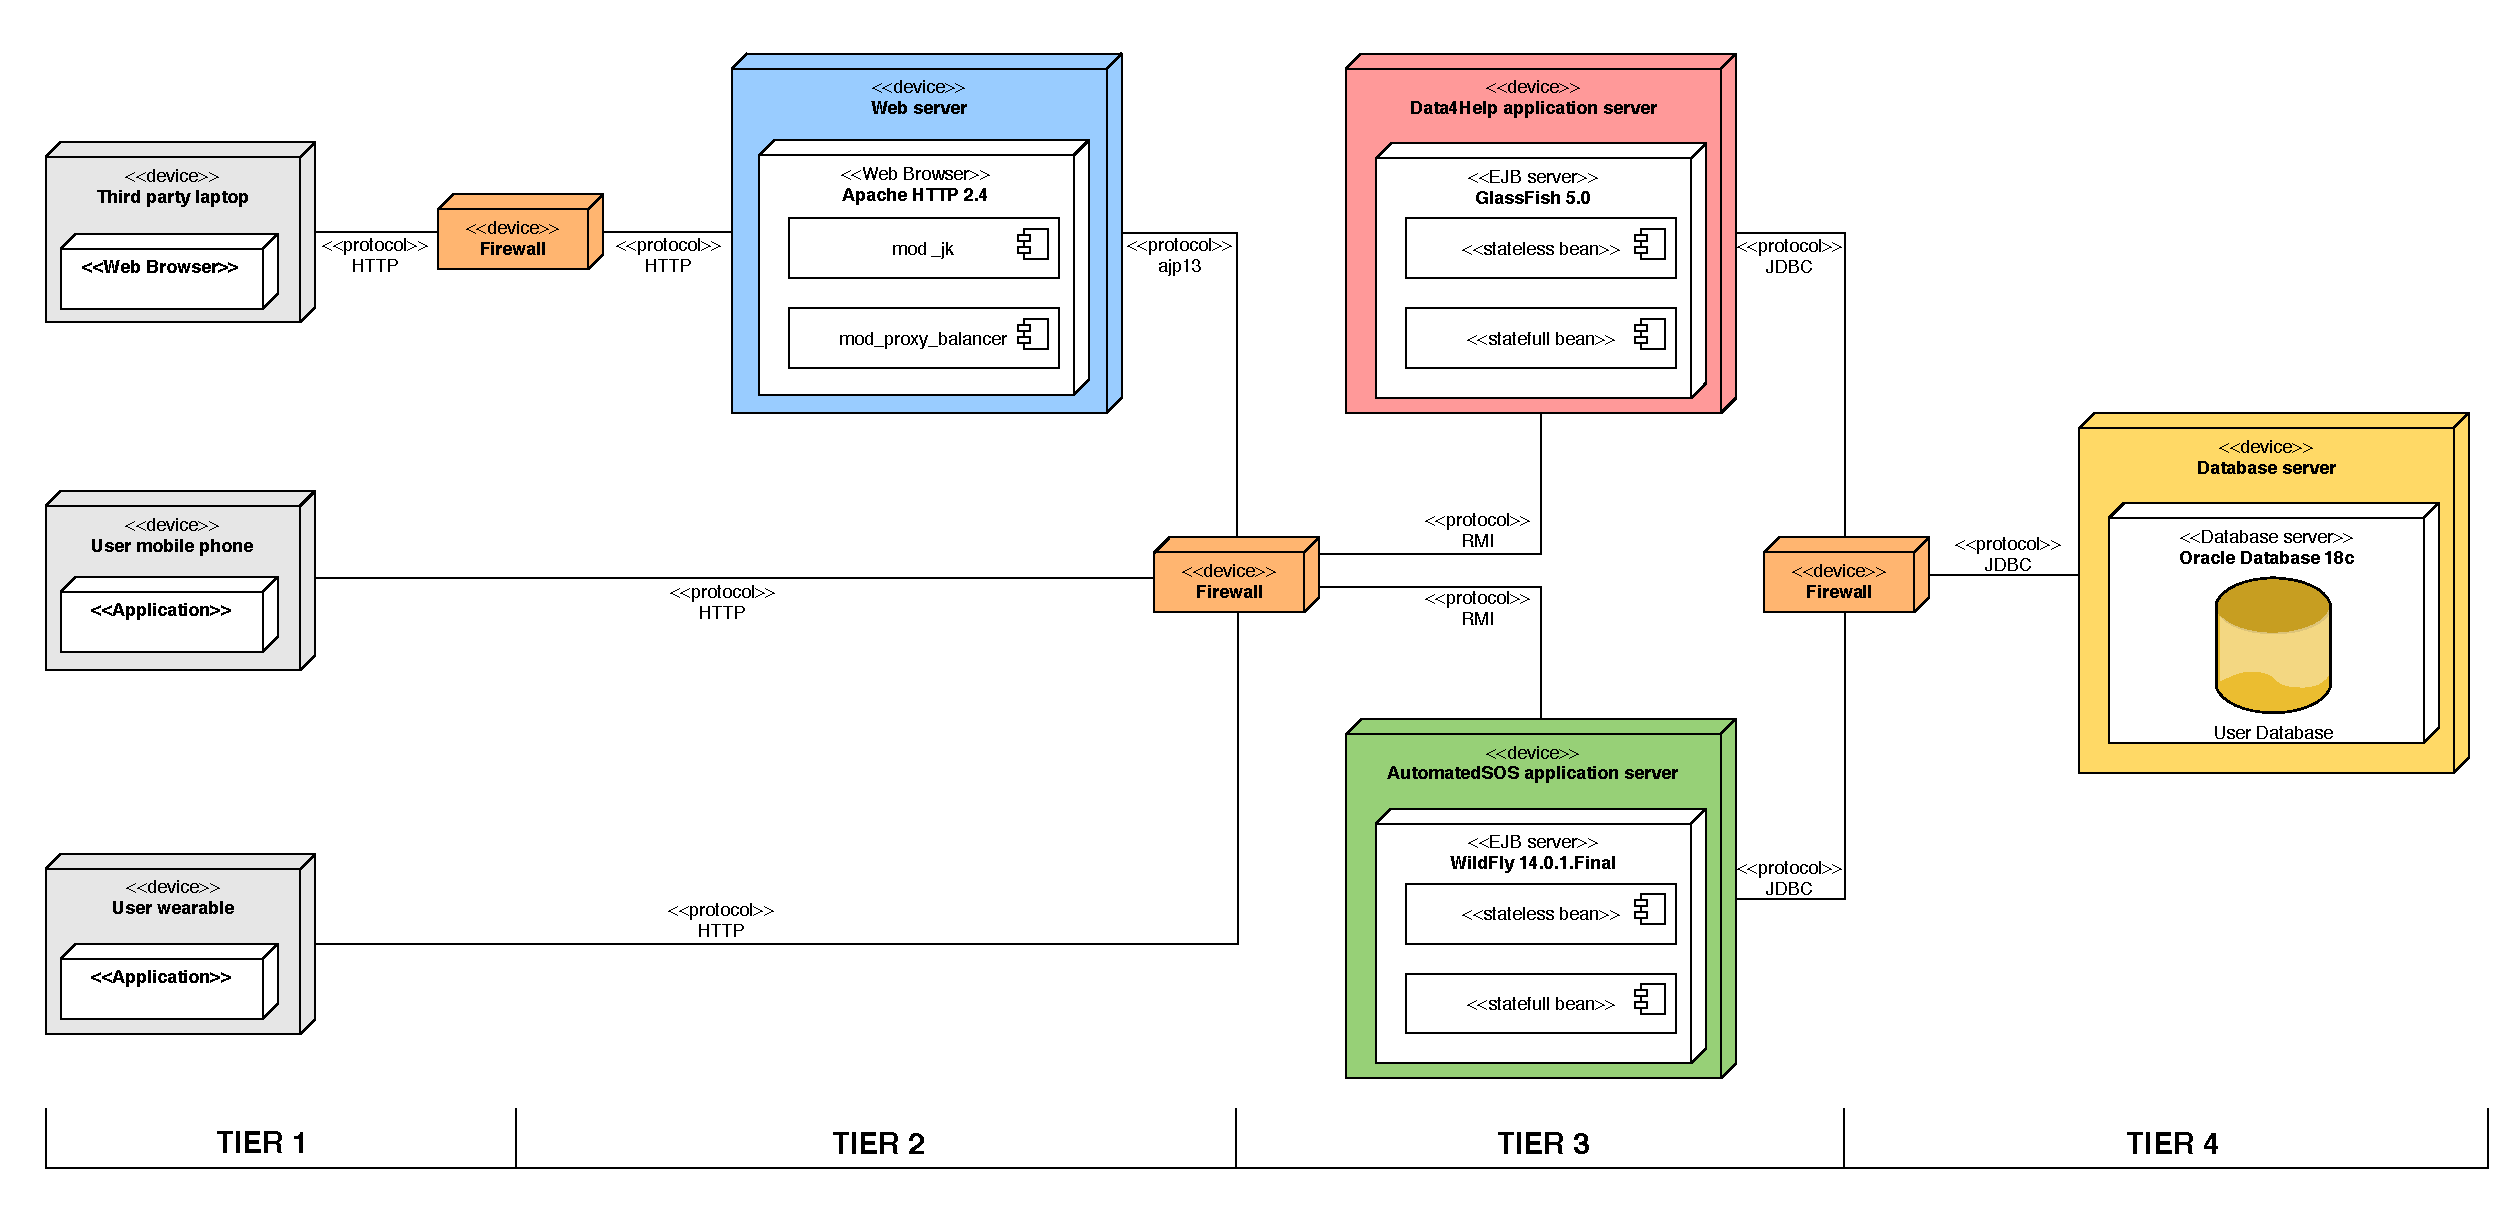
\includepdf[angle=90]{pdfs/Deployment_view.pdf}
\end{landscape}

\hypertarget{RV}{\section{Runtime View}}
This section illustrates the phases of the main interactions that happen during the use of the system. Using several Sequence Diagrams, we illustrated the communications between the logic components.\\
Even though we tried to describe the processes in the most clear and detailed way, these diagram remains a high-level description of the interactions flows. Therefore, all of the parameters and methods that appear in these Sequence Diagrams may do not correspond exactly to the ones in the actual implementation of the components.\\
In the following Sequence Diagrams we cover all the possible interactions between each component. We grouped all the Sequence Diagram that belong to the same flow of activities, since for obvious reasons we had to decomposed them in sub-sequence to fit them into this document.
The diagrams presented below cover all these situations:
\begin{itemize}
    \item Registration of a user(which is identical to the registration of a third party, so we omit this last one) : \underline{Figure \ref{RV1}}
    \item Login of a user(which is identical to the login of a third party, so we omit this last one) : \underline{Figure \ref{RV2}}
    \item Third party make an individual request :\\ \underline{Figure \ref{RV1}}, \underline{Figure \ref{RV3}}, \underline{Figure \ref{RV4}}, \underline{Figure \ref{RV5}}, \underline{Figure \ref{RV6}}, \underline{Figure \ref{RV7}}
    \item Third party make a group request :  \underline{Figure \ref{RV8}}
    \item AutomatedSOS analysis health parameters and an anomaly occurs:\\ \underline{Figure \ref{RV9}},  \underline{Figure \ref{RV10}},  \underline{Figure \ref{RV11}}
    
\end{itemize}

\begin{figure}[ht]
    \makebox[\textwidth]{
        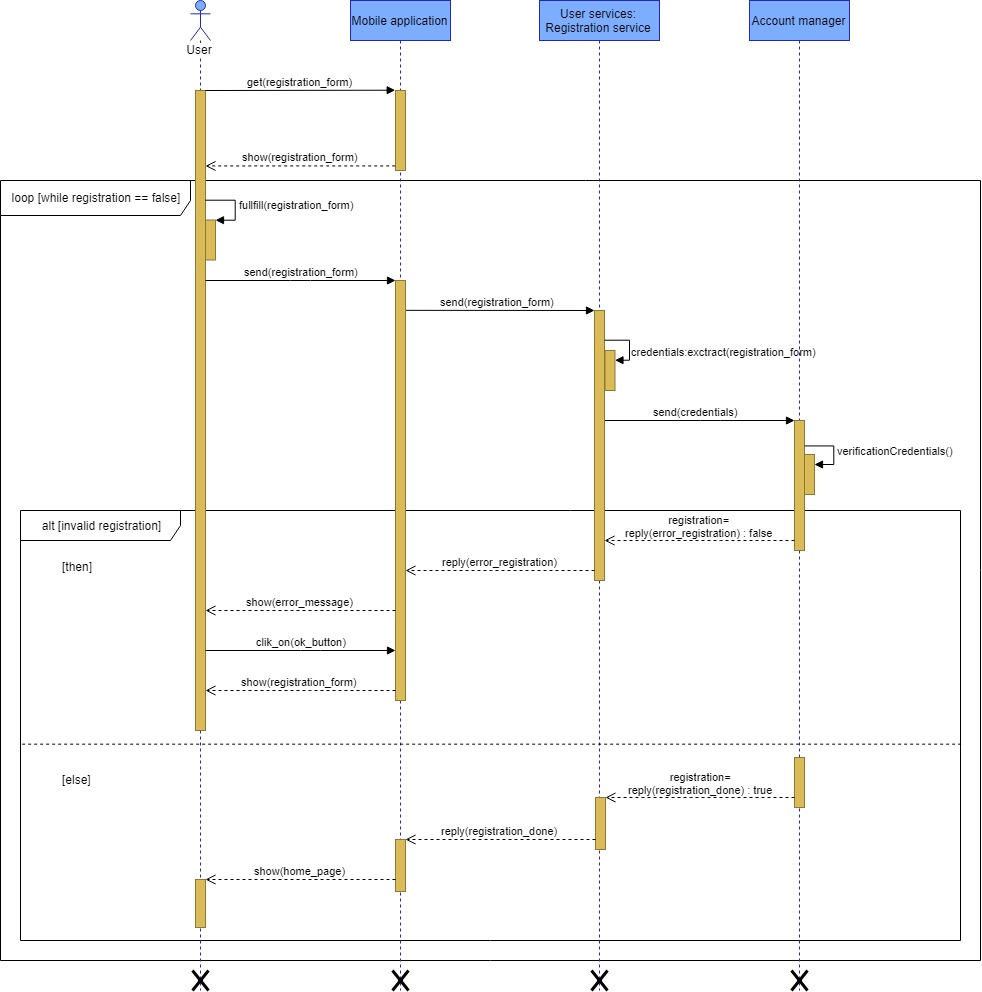
\includegraphics[width=1.3\linewidth]{images/RuntimeDiagrams/Registration.jpg}
    }
    \caption{Data4Help - Registration of a user.}
    \label{RV1}
\end{figure}

\begin{figure}[ht]
    \makebox[\textwidth]{
        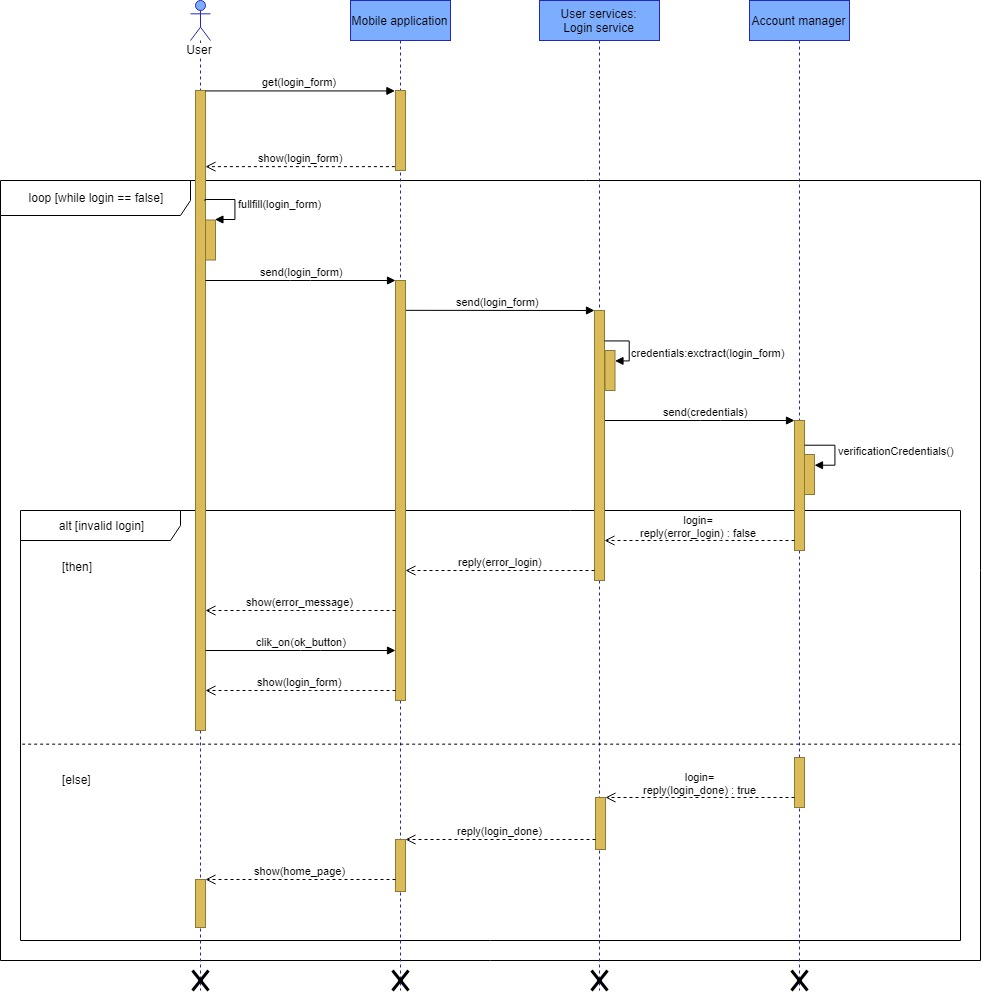
\includegraphics[width=1.3\linewidth]{images/RuntimeDiagrams/Login.jpg}
    }
    \caption{Data4Help - Login of a user.}
    \label{RV2}
\end{figure}

%individual request(from here)
\begin{figure}[ht]
    \makebox[\textwidth]{
        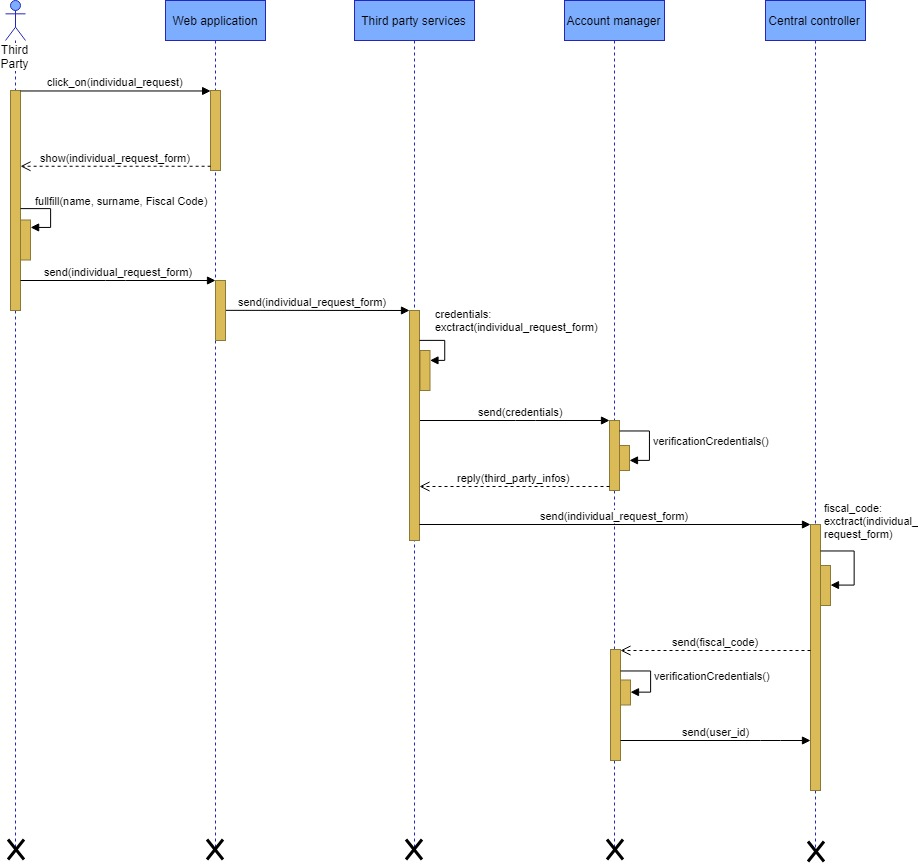
\includegraphics[width=1.3\linewidth]{images/RuntimeDiagrams/IndividualRequest1.jpg}
    }
    \caption{Individual request - Third party make an individual request.}
    \label{RV3}
\end{figure}

\begin{figure}[ht]
    \makebox[\textwidth]{
        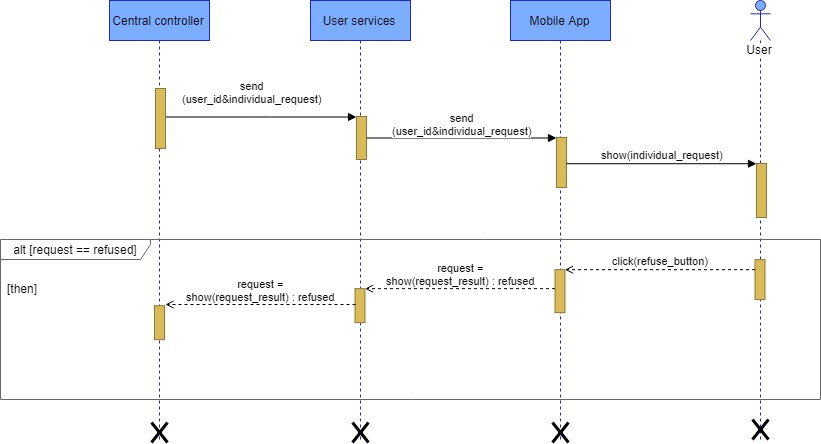
\includegraphics[width=1.3\linewidth]{images/RuntimeDiagrams/IndividualRequest2.jpg}
    }
    \caption{Individual request - The individual request is forwarded to the user and he/she refuses it.}
    \label{RV4}
\end{figure}

\begin{figure}[ht]
    \makebox[\textwidth]{
        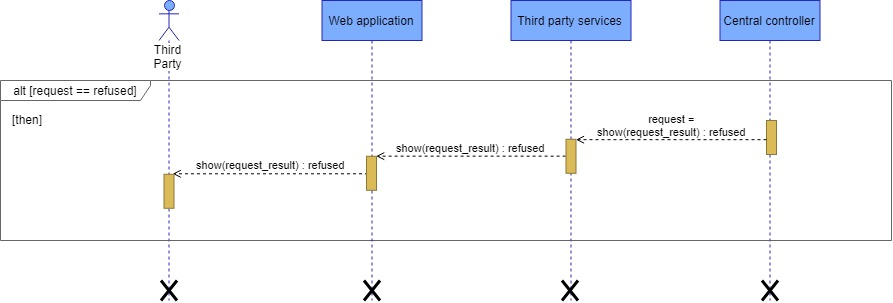
\includegraphics[width=1.3\linewidth]{images/RuntimeDiagrams/IndividualRequest3.jpg}
    }
    \caption{Individual request - The reply is sent to the third party.}
    \label{RV5}
\end{figure}

\begin{figure}[ht]
    \makebox[\textwidth]{
        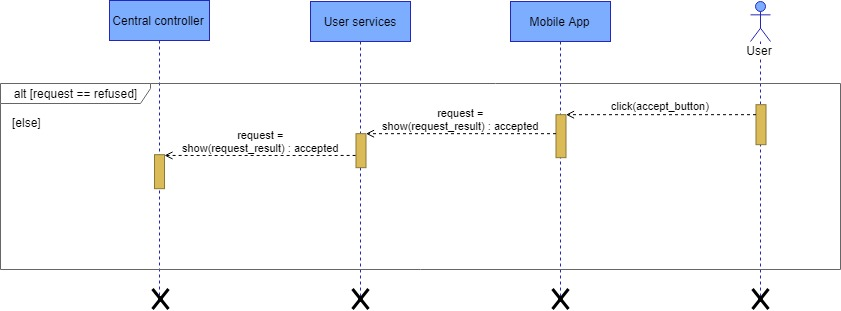
\includegraphics[width=1.3\linewidth]{images/RuntimeDiagrams/IndividualRequest4.jpg}
    }
    \caption{Individual request - The user accepts the request.}
    \label{RV6}
\end{figure}

\begin{figure}[ht]
    \makebox[\textwidth]{
        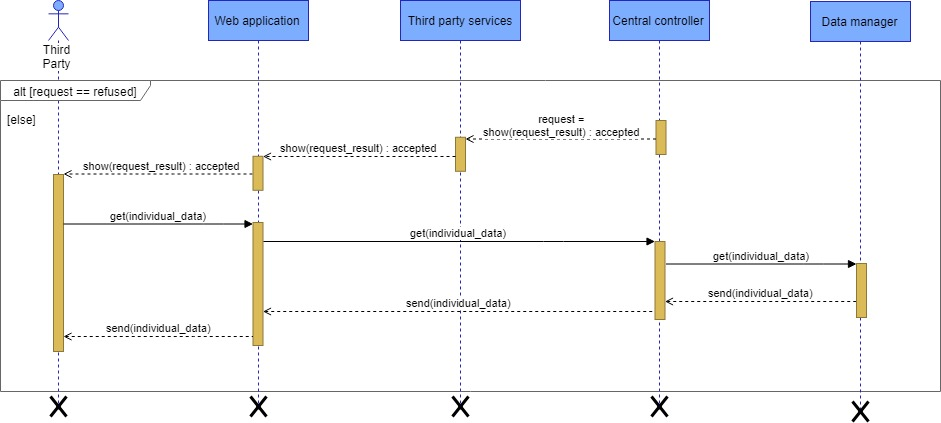
\includegraphics[width=1.3\linewidth]{images/RuntimeDiagrams/IndividualRequest5.jpg}
    }
    \caption{Individual request - The reply and the individual data are sent to the third party who requested them.}
    \label{RV7}
\end{figure}
%individual request(up to here)

\begin{figure}[ht]
    \makebox[\textwidth]{
        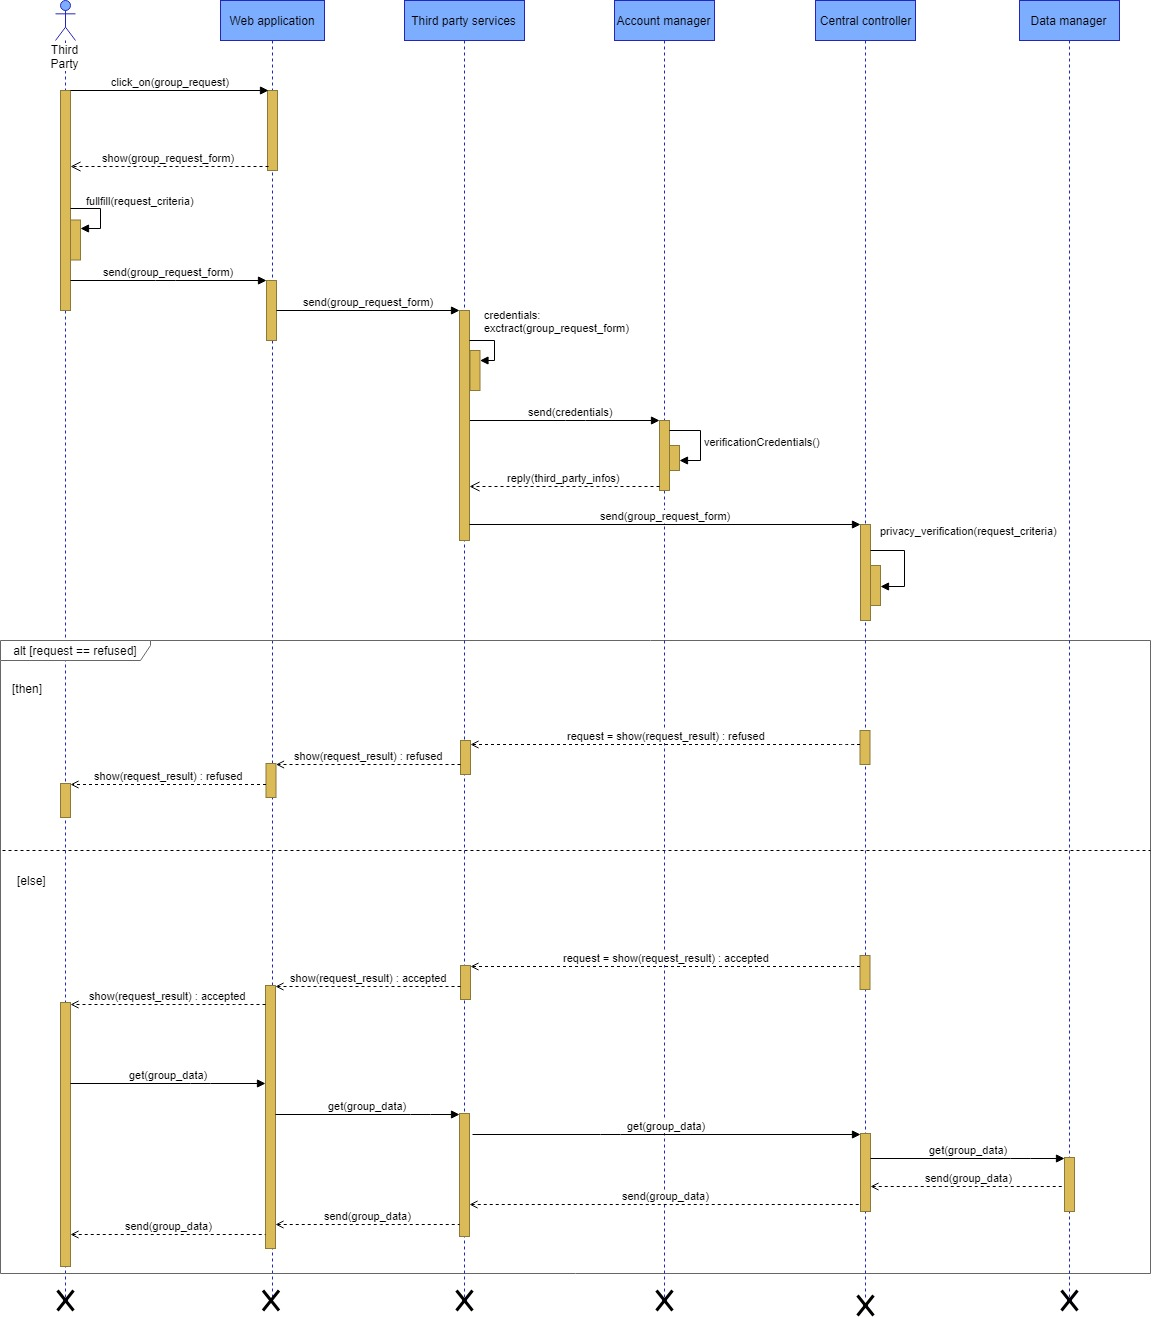
\includegraphics[width=1.3\linewidth]{images/RuntimeDiagrams/GroupRequest.jpg}
    }
    \caption{Data4Help - Third party make a group request.}
    \label{RV8}
\end{figure}

\begin{figure}[ht]
    \makebox[\textwidth]{
        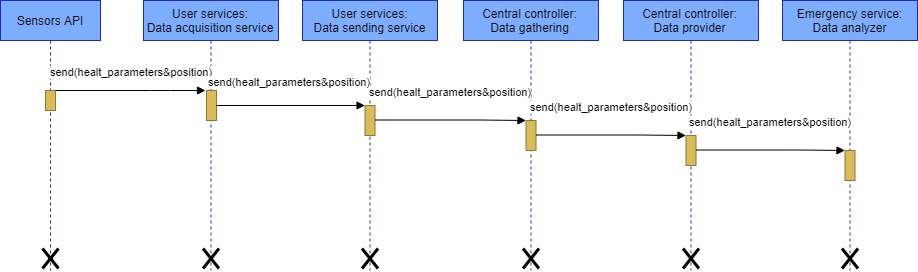
\includegraphics[width=1.3\linewidth]{images/RuntimeDiagrams/Ambulance1.jpg}
    }
    \caption{AutomatedSOS - real-time data acquisition.}
    \label{RV9}
\end{figure}

\begin{figure}[ht]
    \makebox[\textwidth]{
        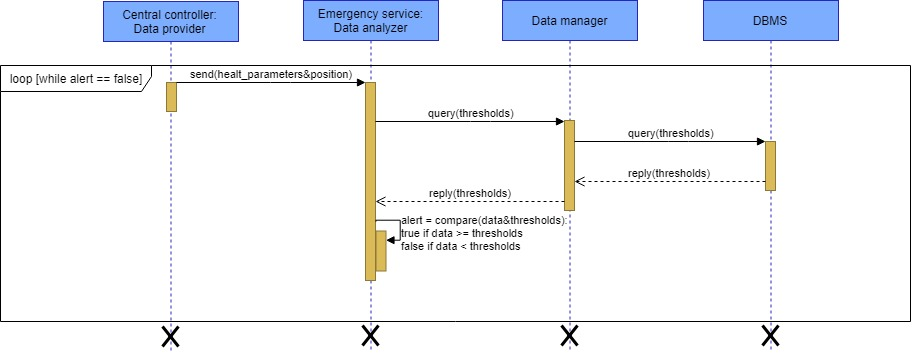
\includegraphics[width=1.3\linewidth]{images/RuntimeDiagrams/Ambulance2.jpg}
    }
    \caption{AutomatedSOS - real-time data analysis.}
    \label{RV10}
\end{figure}

\begin{figure}[ht]
    \makebox[\textwidth]{
        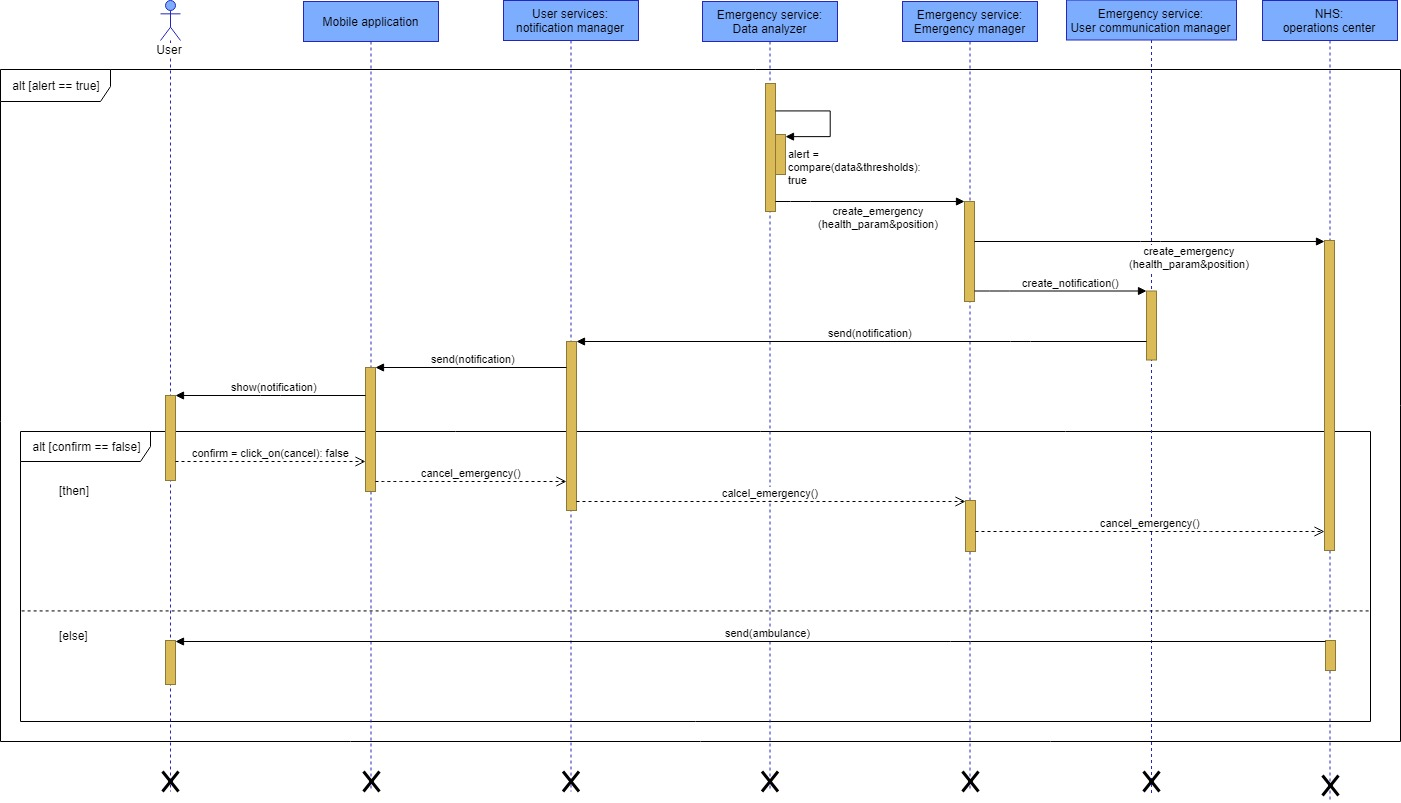
\includegraphics[width=1.3\linewidth]{images/RuntimeDiagrams/Ambulance3.jpg}
    }
    \caption{AutomatedSOS - an emergency occurs.}
    \label{RV11}
\end{figure}

\clearpage
\section{Component Interfaces}
The diagrams showed below list the main methods that forms the components interfaces.\\

Since the Central Controller behaves as intermediate between users (collection of data) and third parties (transfer of these data), the component offers interfaces that serve the communication with both parties.
In particular, the Individual Request Manager offers method for the addition of a request by a third party and the response to that request by the user. (AGGIUNGERE AL DIAGRAMMA)\\

The Third Party and User services offer all the methods responsible for the interaction between the client applications and the back-end. Thanks to these components, all the different implementations of the presentation tier can interact with the same interface.\\
Examples of methods offered by the Third Party Services regards the sending of a request and the access to users' data. Examples of methods offered by the User Services are regards the response to an incoming request and the data acquisition from the device.\\

The emergency service provide the methods to collect(AGGIUNGERE AL DIAGRAMMA) and analyze health data, generate and send emergency notification to the NHS and communicate with the user(secondo me c'è un errore nel diagramma).\\
\clearpage

\begin{figure}
    \centering
    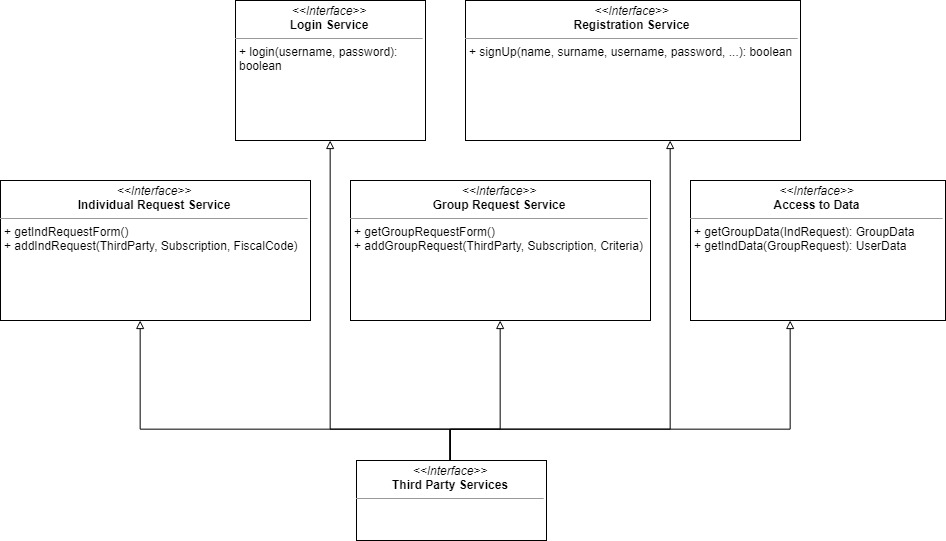
\includegraphics[width=300pt]{images/CompInterfaces/Component_interfaces3.jpg}
    \caption{Component Interface}
\end{figure}

\begin{figure}
    \centering
    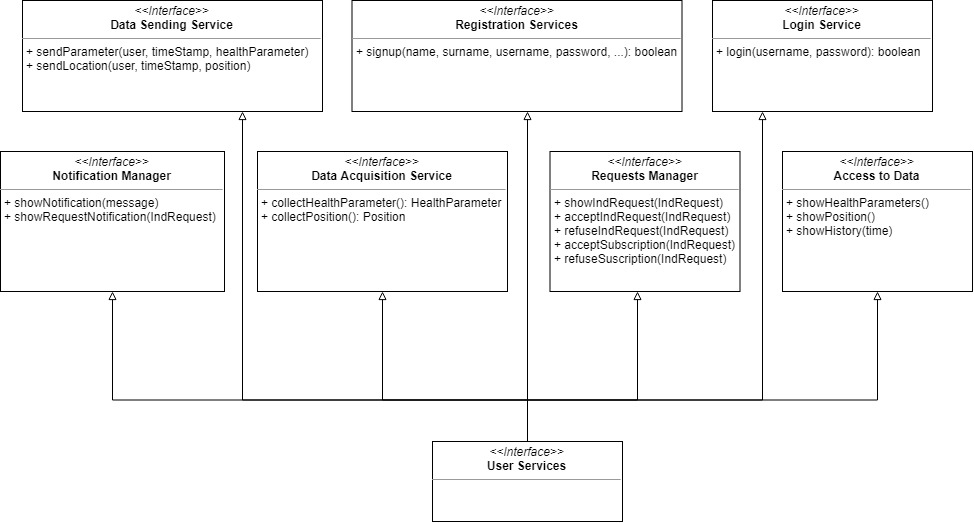
\includegraphics[width=300pt]{images/CompInterfaces/Component_interfaces4.jpg}
    \caption{Component Interface}
\end{figure}


\begin{figure}
    \centering
    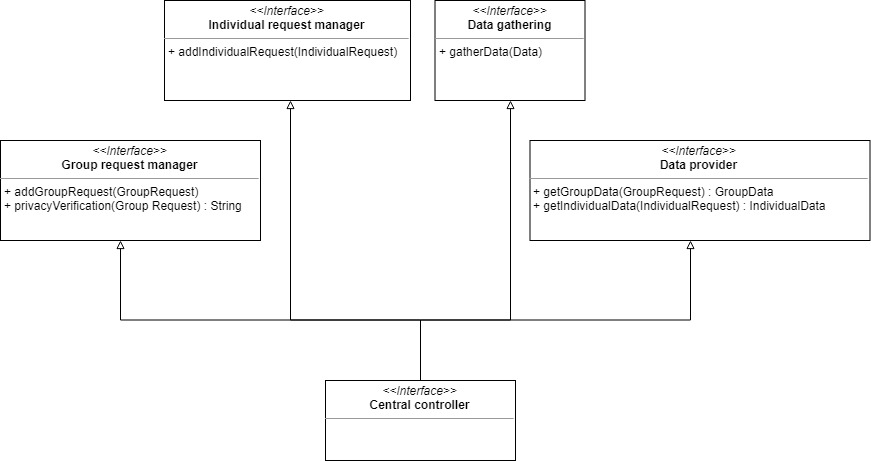
\includegraphics[width=300pt]{images/CompInterfaces/Component_interfaces1.jpg}
    \caption{Component Interface}
\end{figure}

\begin{figure}
    \centering
    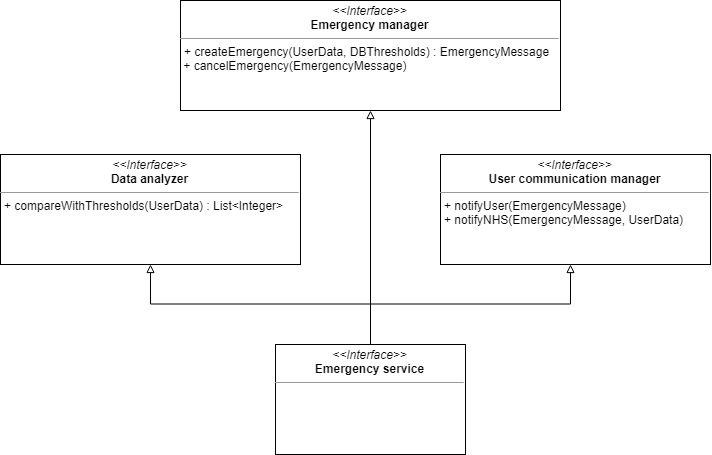
\includegraphics[width=300pt]{images/CompInterfaces/Component_interfaces2.jpg}
    \caption{Component Interface}
\end{figure}


\clearpage

\section{Selected Architectural Styles and Patterns}
\begin{itemize}
    \item \textbf{Model-View-Controller:} it's a very common design pattern, that separates the architecture into three communicating components. The Controller acts performs actions on the Model, using inputs from the View. The Model contains the application's data structures and the View gives an external representation of them.\\ 
    Using the MVC pattern promotes the code reuse and avoid the coupling between the data and their representation. This pattern is particularly appropriate for complex systems such as Data4Help and AutomatedSOS, that will be deployed in multiple physical nodes and will provide several types of views to their users.  
    \item \textbf{Service Oriented Architecture:} we designed the system's components as a set of services that connects with each other through a communication protocol. Viewing each component as a service gives the advantages of abstracting its functions to the highest level and see the module as a independent black box.\\
    A SOA enhances the modularity and maintainability of the system. It also promotes the creation of robust and complete interfaces for each component.
    \item \textbf{Proxy Pattern and Facade Pattern:} we used these patterns mainly for the interactions between the back-end and the client applications. The proxy pattern provides an intermediate object that substitute for the real subject of a communication, while controlling that the input is valid and the access is appropriate. The facade pattern implements a simple interfaces for the access of the back-end system and also acts as an adapter for the information exchanges in the messages. We use these patterns to create an interface between clients and the central system that could be simple to access, secure and that could minimize the dependencies between modules.
    \item \textbf{Publish/Subscribe Pattern:} it is closely related to the MVC pattern. This architectural style offers great scalability and it's fundamental to ensure satisfying performances in an event-based system. Using this pattern will consent to send users' data as soon as they are collected and to notify an emergency as soon as it's detected. 
    \item \textbf{Factory pattern (software design pattern):} a factory object provides a public method for creating other objects, while hiding the actual creation process. The factory pattern promoted the overall encapsulation in the code base.
    \item \textbf{Strategy pattern (software design pattern):} allows the creation of a set of encapsulated algorithms and the selection of one of them at run-time. This pattern is one of the most common in OOP and promotes encapsulation and polymorphism.
    \item \textbf{Adapter pattern (software design pattern):} used to adapt two different interfaces. This pattern is particularly useful for the integration between AutomatedSOS and each country NHS. A more detailed description of its usage will be given in the next paragraph. 
\end{itemize}

\section{Other Design Decisions}

\begin{itemize}
    \item \textbf{Google Maps API:} to represent current positions and daily routes we will use the maps API offered by Google. This API is the common standard because of its quality and current updates. Google Maps offers an interface for JavaScript, Android and iOS development.
    \item \textbf{Sensors API and healthKit:} to collect data from users' device we will with the API offered by Android and iOS platforms: Sensors API and healthKit.
    \item \textbf{AutomatedSOS and Data4Help integration:} when designing AutomatedSOS, we followed two main guide lines: promoting the code reuse as much as possible and keeping the central logic of the application independent from Data4Help's components.
    Given these objectives, we designed AutomatedSOS as an independent service, built on-top of Data4Help platform. 
    The two apps shares the same account management system, so whenever a user registers to AutomatedSOS he/she is also a Data4Help user.\\
    AutomatedSOS core module (\hyperlink{ES}{ \underline{Emergency Service}}) exploits Data4Help's Data Provider to obtain users' data in real time.
    Placing the two system's logic in distinct logic modules favors a distributed deployment of the back-end and a correct load balance.
    In terms of reliability, a failure in AutomatedSOS does not affect Data4Help operations (the vice versa is not true, for obvious reasons).
    \item \textbf{Interaction with the NHS:} AutomatedSOS will be hopefully adopted in several countries, that have significantly different National Health Institutions, First Aid services and unit of measurement for the health parameters.\\
    An efficient integration between the system and the local NHS is the fundamental requirement for the success of an application that deals with its users' lives.\\
    The existence of many differences between the countries forces the design to be adapted to each specific NHS. In order to do so, the NHS Adapter is the interface component responsible for the translation between the system and the local Operations Center.
    To give an high-level description: if a country offers an API to send a digital message to the Operations Center, the NHS Adapter will connect to it; if such an API does not exists, the NHS adapter will call 911 telephone number and read the emergency message to the operator with an artificial voice.
    (CAMBIARE DIAGRAMMI)
\end{itemize}

\chapter{User Interface Design}
\hypertarget{MK}{\section{Mock-up Interfaces}}
We think that the success of one application strongly depends on his user-friendly graphic design. According to this we propose, both in the RASD and in the DD documents, some mockups trying to be as intuitive and satisfactory as possible.\\
We also want to offer the possibility to run the two applications on a large number of devices. 
In order to facilitate the diffusion of the Data4Help and AutomatedSOS applications, we want them to run properly on different hardware platforms: personal computers, mobile phones and also wearable devices. In the RASD document we have already presented some UIs that accomplish this multi-platform requirement.
Moreover, we designed our application with the purpose to be resizable, so that it can adapt to screens of different dimension.\\
In the RASD document are illustrated 12 different mockups that represent different parts of Data4Help and AutomatedSOS applications. Here we want to introduce 4 new mockups, to increment and complete the overview of the graphic appearance of the two applications. \\
In particular, in this document, we focused on:
\begin{itemize}
    \item \textbf{Menu:}
    from this page, the user can reach all the pages of Data4Help application by clicking on the respective item.
    \item \textbf{Home page:}
    here the user can see his real-time position on a map(based on Google Maps) and his real-time health parameters.
    Moreover he/she can see the notifications for the new requests.
    \item \textbf{Manage requests:}
    in this page the user can accept or decline the requests for his/her data and he/she can interrupt the subscriptions to updated data previously accepted.
    \item \textbf{History:}
    by selecting a time interval, the user can see the average value of his/her health parameters and he/she can also observe his historic route.
\end{itemize}
\clearpage
\begin{figure}[ht]
    \centering
    \begin{subfigure}[t]{0.38\linewidth}
        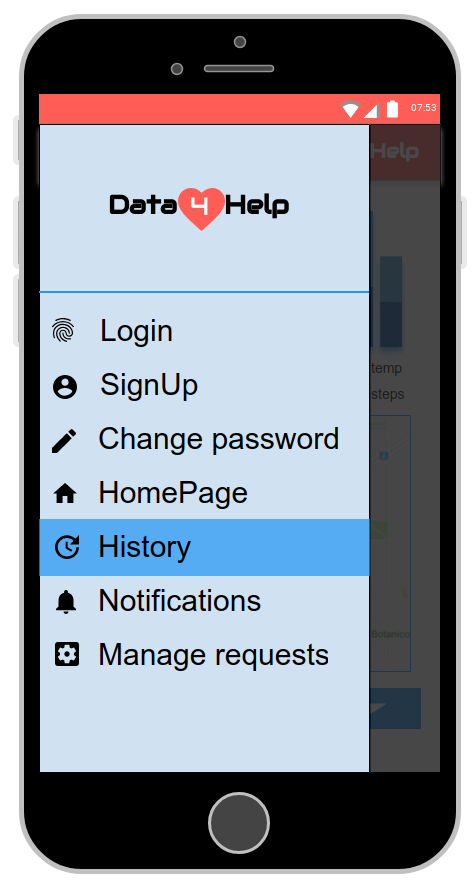
\includegraphics[width=\linewidth]{images/Mockup/Menu.png}
        \caption{Data4Help Menu.}
    \end{subfigure} \hfil \hfil \hfil
    \begin{subfigure}[t]{0.38\linewidth}
        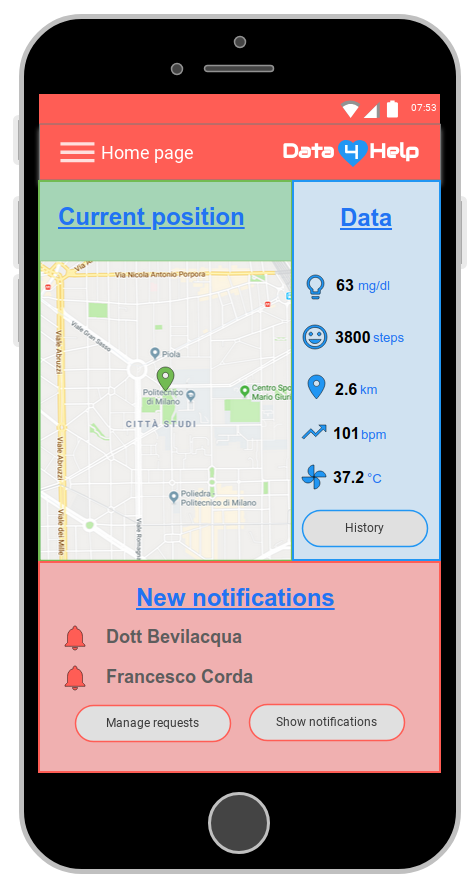
\includegraphics[width=\linewidth]{images/Mockup/Home_page.png}
        \caption{Data4Help Home Page.}
    \end{subfigure}
    
  \begin{subfigure}[t]{0.38\linewidth}
    \centering
    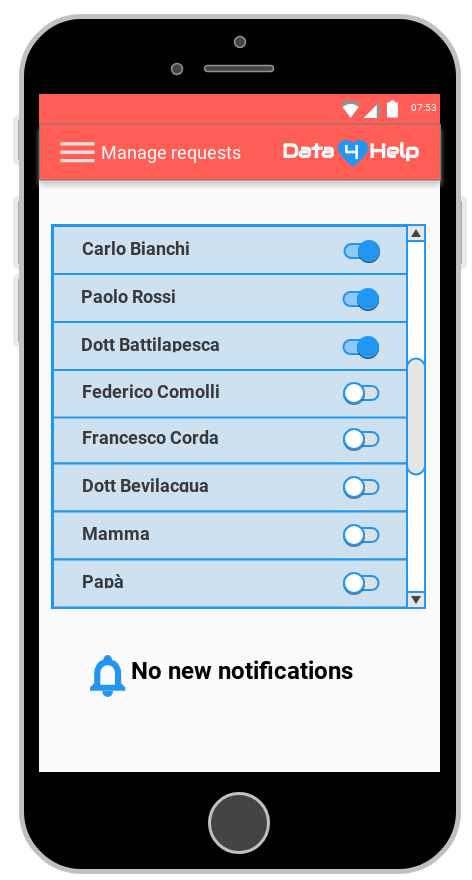
\includegraphics[width=\linewidth]{images/Mockup/Manage_requests.png}
    \caption{User manages his requests.}
  \end{subfigure} \hfil \hfil \hfil
  \begin{subfigure}[t]{0.38\linewidth}
    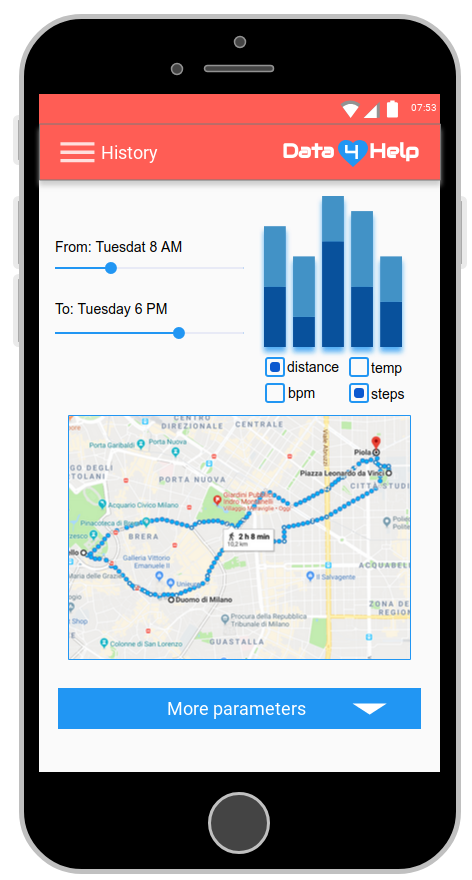
\includegraphics[width=\linewidth]{images/Mockup/History.png}
    \caption{User observes his historical data.}
  \end{subfigure}
\end{figure}
\clearpage

\section{User Experience Diagrams}
We have already presented how the different screens of our application will look like, showing some comprehensive mockups in the \hyperlink{MK}{\underline{section above}} and in the RASD document. However they are in some way \say{static}, and just by observing all the presented interfaces it's not possible to understand how they interact with each other.
For this purpose, here are presented three different User Experience diagrams with the intention to cover all the possible applications of the system (web, wearable or mobile).
The diagrams presented here and in the following pages are preceded by a short introduction.\\ \\
The first one describes the User experience with the mobile application (and also partly with the wearable application). The first screen that User has to face is the Login page. From here the user can reach the Registration page or, if it has already an account, the Home page. From this last page, he/she finally can reach the Manage Requests, the Accept/Decline Requests or the History screen.
\begin{figure}[ht]
    \centering
    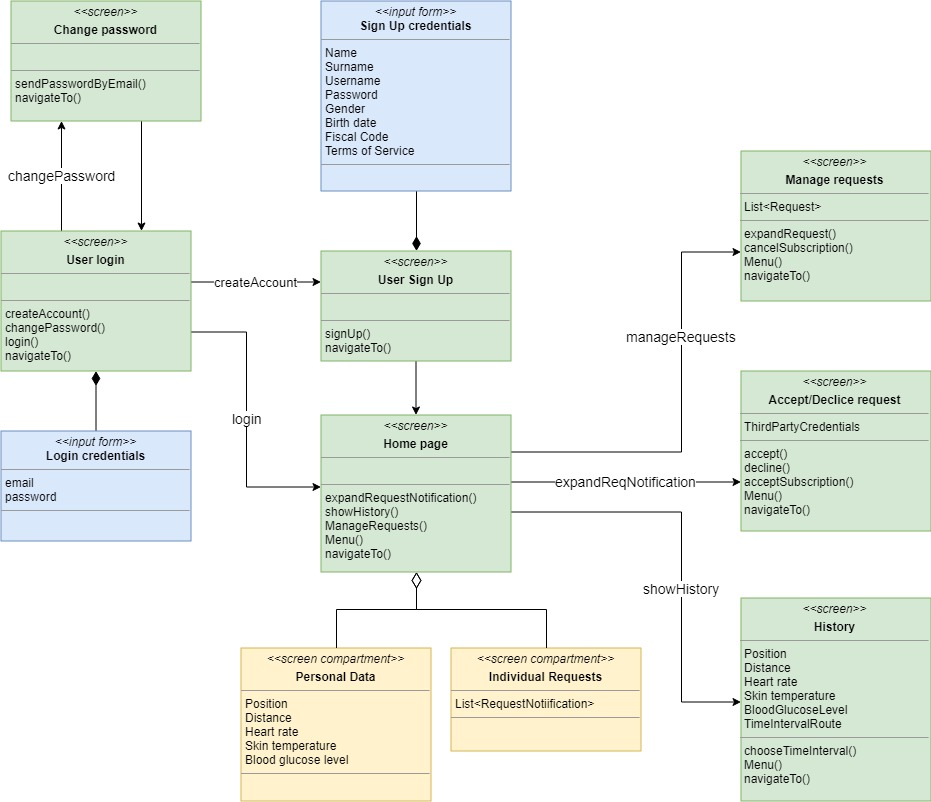
\includegraphics[width=300pt]{images/UX/UX_Diagram1.jpg}
    \caption{Data4Help - User experience}
    \label{UX1}
\end{figure}
\clearpage
\noindent The second diagram describes the experience of the third party through the mobile application(or maybe also through the Web application). The first page that he/she has to face is obviously the login screen, from which he/she can reach the Registration or the Home pages. Finally, from this last screen the third party can reach the Create Group Request, Create Individual Request and the Requested Data pages.
\begin{figure}[ht]
    \centering
    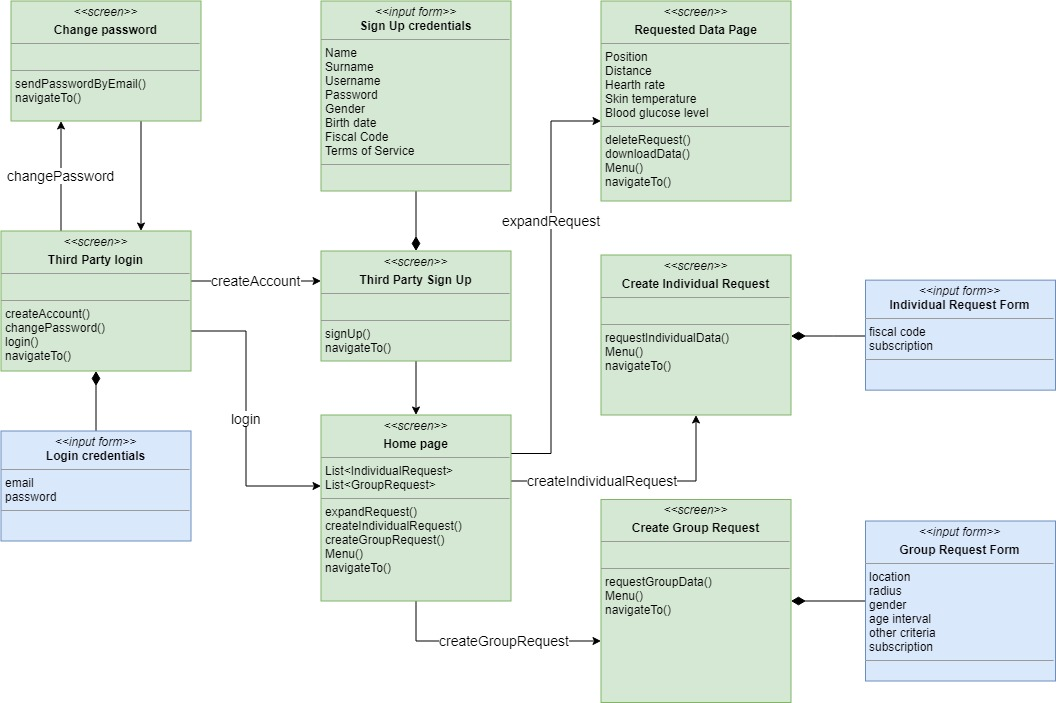
\includegraphics[width=300pt]{images/UX/UX_Diagram2.jpg}
    \caption{Data4Help - third party experience}
    \label{UX2}
\end{figure}
\clearpage
\noindent This last diagram illustrates the experience of a User through the AutomatedSOS mobile application (and also partly through the wearable application). As in the other UXs, the first page that the user has to face is the Login page, followed by the Registration or Home pages. The last available page of this application is the Emergency screen, that appears instead of the home page when an emergency is detected.
\begin{figure}[ht]
    \centering
    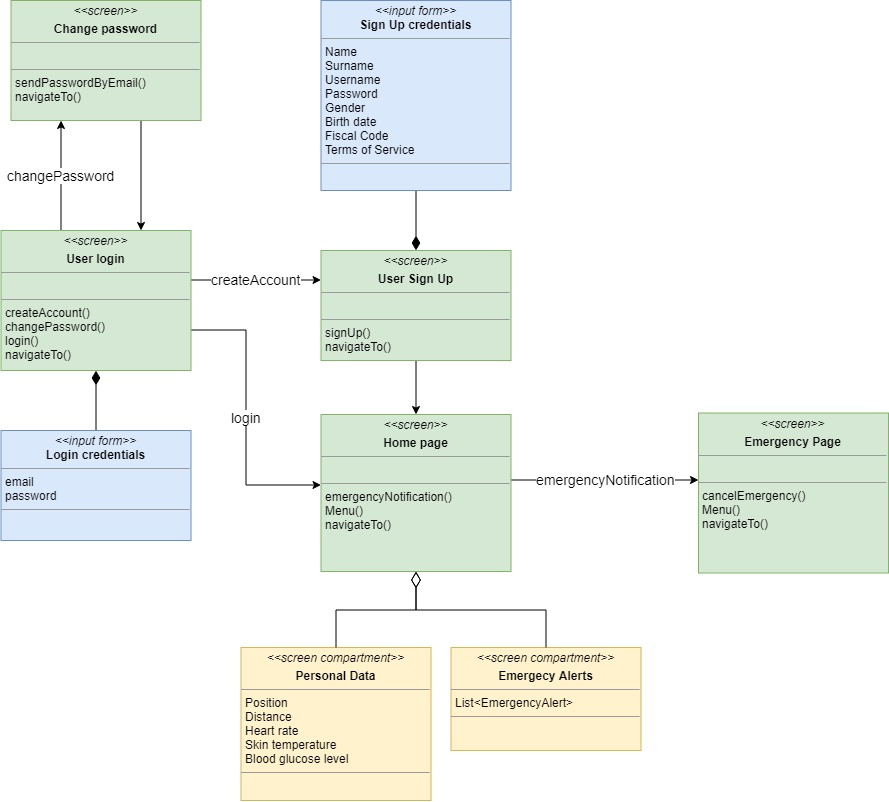
\includegraphics[width=300pt]{images/UX/UX_Diagram3.jpg}
    \caption{AutomatedSOS - User experience}
    \label{UX3}
\end{figure}
\clearpage

\section{Boundary Control Entity Diagrams}
In the last section of the chapter focused on the User Interfaces we want to reach a further level of detail.\\
We showed all the available pages of our applications-to-be and how the user and the third party can navigate through them.\\
Here we want to illustrate how the interactions of a User/Third Party with respective applications are managed by the \say{Controller} and how they affect the \say{Model}.
In the following diagrams we refer to the Model-View-Controller design pattern, which guarantees the correct separation between the presentation of the application and its core logic.\\
The entities on the left are intended as part of the View of our applications-to be, the entities on the right are part of the Model and, for last, the ones at the center represent the Controller.

\begin{figure}[ht]
    \centering
    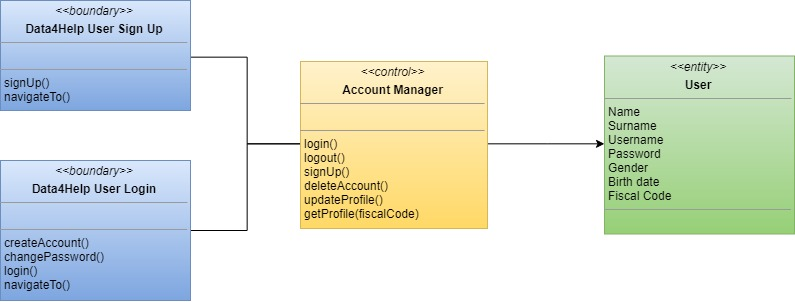
\includegraphics[width=300pt]{images/BCE/BCE_Diagrams1.jpg}
    \caption{User registration and login to Data4Help application.}
    \label{BCE1}
\end{figure}
\begin{figure}[ht]
    \centering
    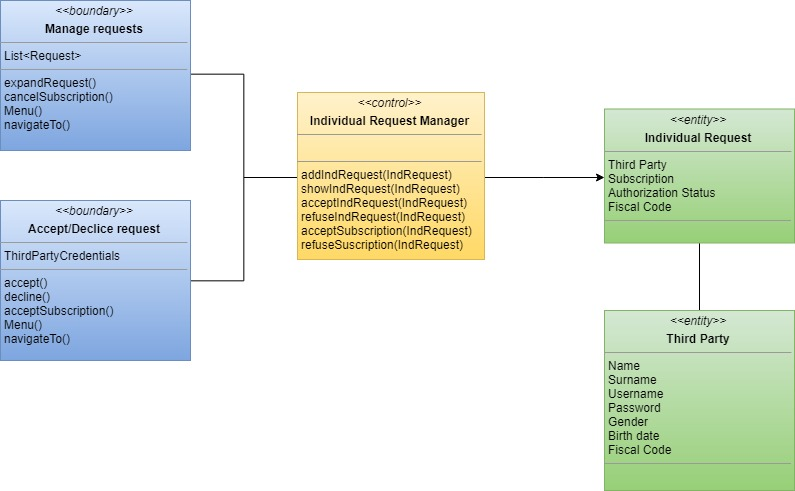
\includegraphics[width=300pt]{images/BCE/BCE_Diagrams2.jpg}
    \caption{The user responds to a request and manages previous requests.}
    \label{BCE2}
\end{figure}
\begin{figure}[ht]
    \centering
    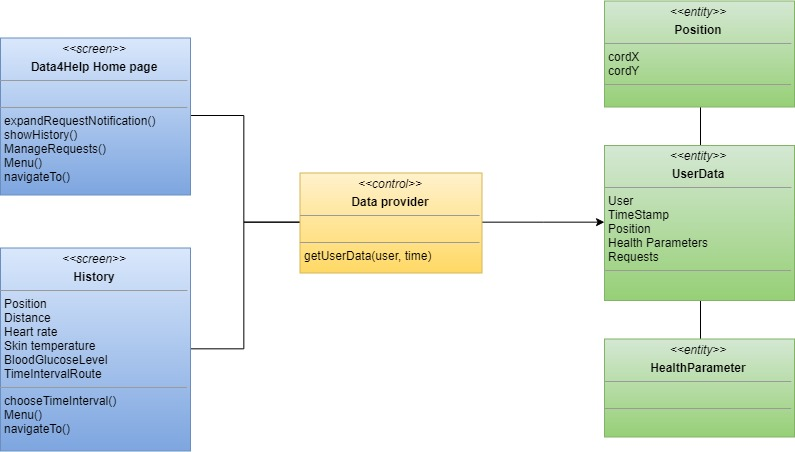
\includegraphics[width=300pt]{images/BCE/BCE_Diagrams3.jpg}
    \caption{The user accesses current or historical personal data.}
    \label{BCE3}
\end{figure}
\begin{figure}[ht]
    \centering
    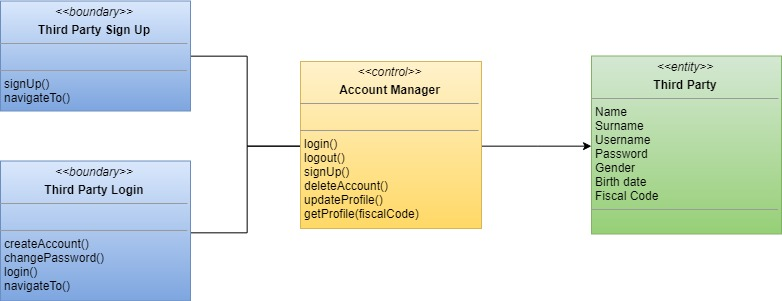
\includegraphics[width=300pt]{images/BCE/BCE_Diagrams4.jpg}
    \caption{Third party registration and login to the Data4Help application.}
    \label{BCE4}
\end{figure}
\begin{figure}[ht]
    \centering
    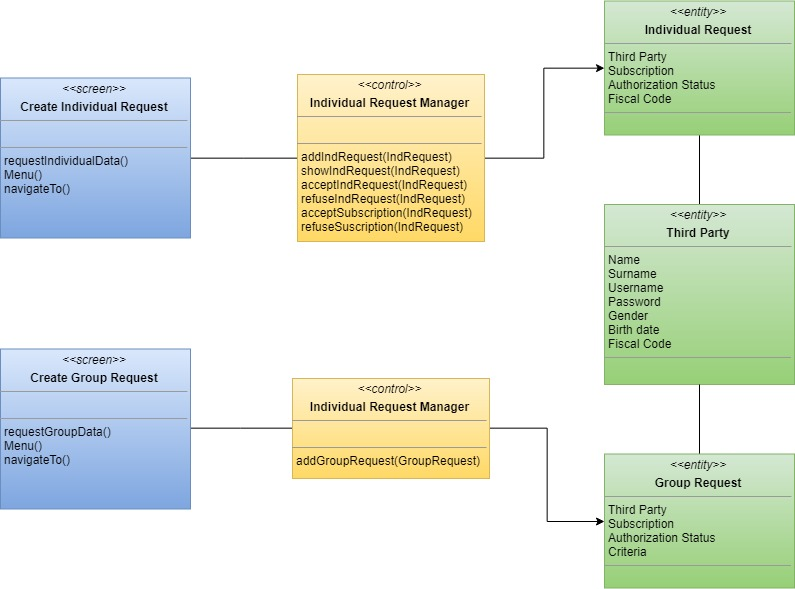
\includegraphics[width=300pt]{images/BCE/BCE_Diagrams5.jpg}
    \caption{A third party creates an individual or group request.}
    \label{BCE5}
\end{figure}
\begin{figure}[ht]
    \centering
    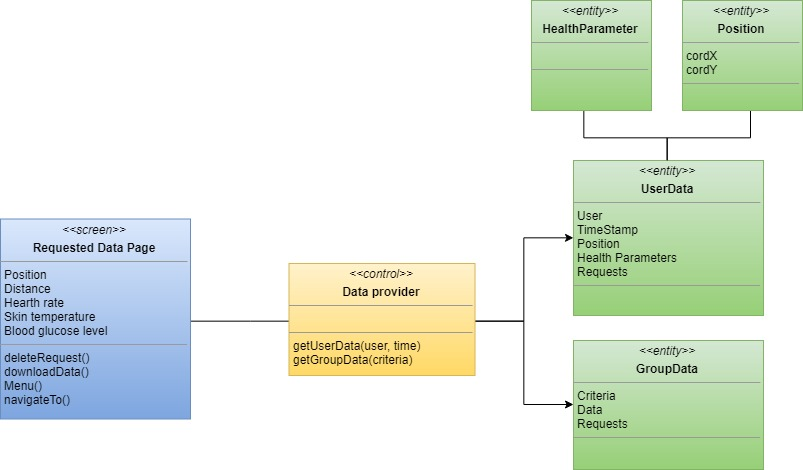
\includegraphics[width=295pt]{images/BCE/BCE_Diagrams6.jpg}
    \caption{A third party obtains the requested data.}
    \label{BCE6}
\end{figure}
\begin{figure}[ht]
    \centering
    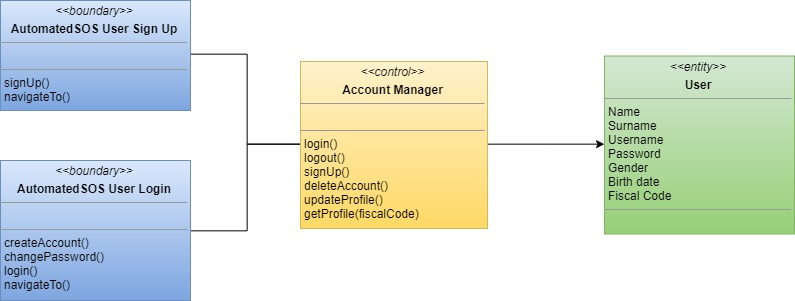
\includegraphics[width=295pt]{images/BCE/BCE_Diagrams7.jpg}
    \caption{User registration and login to AutomatedSOS application.}
    \label{BCE7}
\end{figure}
\begin{figure}[ht]
    \centering
    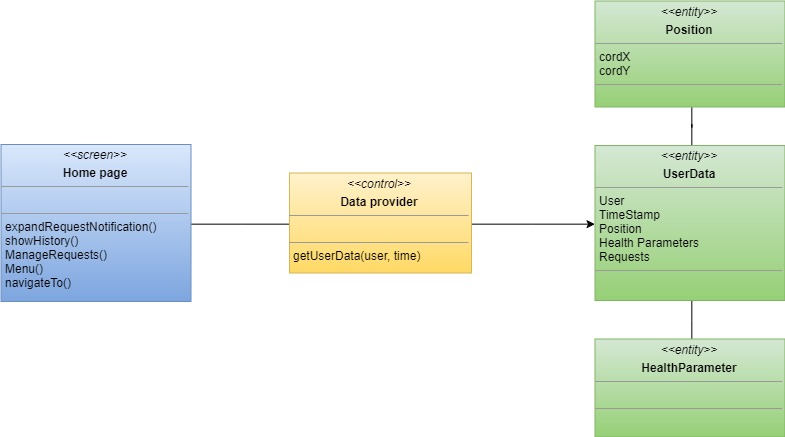
\includegraphics[width=295pt]{images/BCE/BCE_Diagrams8.jpg}
    \caption{A user accesses current personal data.}
    \label{BCE8}
\end{figure}
\begin{figure}[ht]
    \centering
    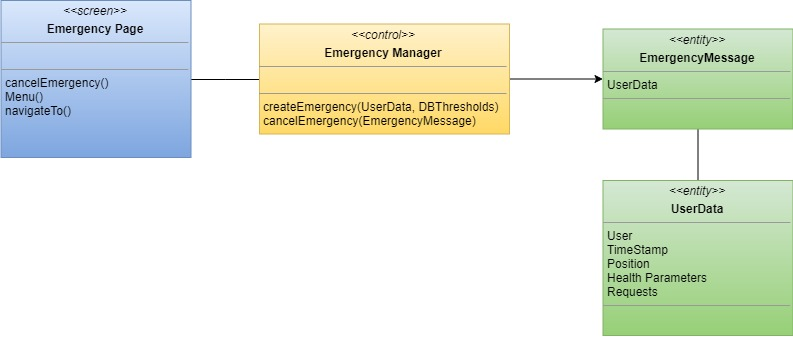
\includegraphics[width=300pt]{images/BCE/BCE_Diagrams9.jpg}
    \caption{Emergency Page activated in case of a health crisis.}
    \label{BCE9}
\end{figure}

\chapter{Requirements Traceability}
\section{Functional Requirements}
The design decisions illustrated in this document have been taken with the purpose to satisfy all the functional requirements listed in the RASD document. In this section, each requirement is mapped into the corresponding design components.
The mapping can be better understood by observing the \hyperlink{RV}{\underline{Runtime view, section 2.5}}, in which is illustrated the sequential order of the interaction between each design component, in order to accomplish the functional requirements.\\
Other important diagrams that integrate the following mapping, are in the\\ \hyperlink{CV}{\underline{Component view, section 2.3}}.

\begin{enumerate} [label={\bf[R\arabic*]}]
    \item \textbf{The system should provide a registration form offering the following mandatory fields: name, surname, SSN or Fiscal Code.}
        \begin{itemize}
            \item Mobile application
            \item User services: Login service
            \item Account manager
        \end{itemize}
    \item \textbf{The system must guarantee that the credentials are unique.}
        \begin{itemize}
            \item Account manager
        \end{itemize}
    \item \textbf{The system must acquire real-time users' positions from the GPS installed on the user's device.}
        \begin{itemize}
            \item GPS API
            \item User services: Data acquisition service
            \item User services: Data sending service
            \item Central controller: Data gathering
        \end{itemize}
    \clearpage
    \item \textbf{The system must collect users' data in specific databases.}
        \begin{itemize}
            \item Central controller: Data provider
            \item Data manager
            \item DBMS
        \end{itemize}
    \item \textbf{The system must acquire real-time users' health parameters from the sensors installed on the user's device.}
        \begin{itemize}
            \item sensors API
            \item User services: Data acquisition service
            \item User services: Data sending service
            \item Central controller: Data gathering
        \end{itemize}
    \item \textbf{Every time that a third party inserts a request for data relative to a Fiscal Code, the system must ask the authorization to the corresponding user.}
        \begin{itemize}
            \item User services: Request manager
            \item Mobile application
        \end{itemize}
    \item \textbf{The system must provide a function to allow users to accept or refuse a request for personal data.}
        \begin{itemize}
            \item Mobile application
            \item User services: Requests manager
        \end{itemize}
    \item \textbf{The system should provide a registration form to third parties.}
        \begin{itemize}
            \item Web application
            \item Mobile application
            \item Third party services: Registration service
        \end{itemize}
    \item \textbf{The system must provide a function to allow third parties to request the access to individuals data. The form must require the filling of the SSN or Fiscal Code of the corresponding user.}
        \begin{itemize}
            \item Web application
            \item Mobile application
            \item Third party services: Individual request service
            \item Account manager
            \item Central controller: Individual request manager
            \item User services: Requests manager
        \end{itemize}
    \item \textbf{The system must provide a function to allow third parties to request the access to data of a group of people. The form must offer some selection criteria such as geographical, time, health parameters, movement habits, ecc.}
        \begin{itemize}
            \item Web application
            \item Mobile application
            \item Third party services: Group request service
            \item Account manager
            \item Central controller: Group request manager
        \end{itemize}
    \item \textbf{As soon as a request has been approved, the system must forward the most recent data to the third party applying for them.}
        \begin{itemize}
            \item Web application
            \item Mobile application
            \item Third party services: Individual request service
            \item Third party services: Group request service
            \item Third party services: Access to data
            \item Central controller: Data provider
            \item Central controller: Data gathering
            \item Data Manager
            \item DBMS
        \end{itemize}
    \item \textbf{Data4Help must provide a function to let third parties download the received data.}
        \begin{itemize}
            \item Web application
            \item Mobile application
        \end{itemize}
    \item \textbf{The system accepts a request for anonymous data only if the group composing the data is formed by more than 1000 people.}
        \begin{itemize}
            \item Central controller: Group request manager
        \end{itemize}
    \item \textbf{The system must provide a function that allows to customize the requests for subscription to updated data. The requests must include how long the permission is still valid.}
        \begin{itemize}
            \item Mobile application
            \item Web application
            \item Third party services: Individual request service
            \item Third party services: Group request service
        \end{itemize}
    \item \textbf{The system must provide a function to the corresponding user that allows him/her to accept or refuse the subscription request.}
        \begin{itemize}
            \item User services: Request manager
            \item Mobile application
        \end{itemize}
    \item \textbf{The system must forward in real-time the most recent data to the third parties that subscribed to them.}   
        \begin{itemize}
            \item Web application
            \item Mobile application
            \item Third party services: Individual request service
            \item Third party services: Group request service
            \item Third party services: Access to data
            \item Central controller: Data provider
            \item Central controller: Data gathering
            \item Data Manager
            \item DBMS
        \end{itemize}
\end{enumerate}

\section{Non Functional Requirements}

\chapter{Implementation, Integration and Test Plan}
\section{Implementation Plan}
The implementation of Data4Help and AutomatedSOS systems is carried on taking into consideration some important factors, such as the complexity of each component and its relations with the other ones. Of course, the implementation plan takes into special consideration the core components which are essential for the whole system and are considered as \say{bottleneck}. 
It is important to fix any flaws as soon as it is detected, so that the correction costs in terms of time are kept the lower possible.
The order in which our system is implemented is the following:

\begin{enumerate}
    \item Model
    \item Central Controller
    \item Account Manager
    \item Third party services, User Services
    \item Emergency Service
    \item Web, Mobile and Wearable Applications
\end{enumerate}
\begin{figure}[H]
    \makebox[\textwidth]{
        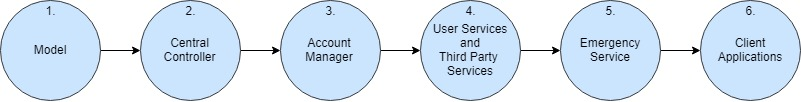
\includegraphics[width=1.3\linewidth]{images/Integration_plan.jpg}
    }
\end{figure}

\subsubsection{Model}
The Model is the first step of the implementation plan, according to its vital role for the whole application.
Since the classes of the Model are used by all the components, it is important that they are ready as soon as possible and are used as a reference. Otherwise each team member would implement the classes of the Model \say{on the fly} when he/she needs them, introducing possible implementation flaws or not using abstraction in a proper way.

\subsubsection{Central Controller}
This component is the logic core of the application. According to this, it requires lot of time to be implemented and, consequently, it is a risky component. It is important that the least possible flaws are inserted during its implementation, since it may have catastrophic consequences in terms of time costs. An important non functional requirement is the fault tolerance and the high throughput. This component may is stressed with lots of requests by each user and third party and it has to react in a short while. For this reason, this component is consider as a \say{bottleneck}.

\subsubsection{Account Manager}
This module allows the sign-up and login of the users and third parties and also is used by the Central Controller when a third party compose a request for data of a specific user. As shown in the \hyperlink{RV}{\underline{Runtime view, section 2.5}}, the third party fills the request form specifying the user's SSN or Fiscal Code and, thanks to the Account Manager, the Central Controller converts it into the corresponding user ID.
This module is used for the login and sign-up processes by both users and third parties and, consequently, it has to use abstraction to achieve this interdependence.

\subsubsection{Third party services, User Services}
This two components allow the interaction between the user application(mobile or wearable) and the third party application(mobile or web), passing through the Central Controller.
They can be implemented together since they are quit similar to each other.
As shown in the \hyperlink{CV}{\underline{Component view, section 2.5}}, the sub-components that allows the login, the registration and the access to data are the same in the two module. 
Regarding to the Individual and the group requests, the Third party services component offers the possibility to create them while the User services component allow the user to manage them.
According to what just said, they are implemented just after the Central Controller and the Account Manager.

\subsubsection{Emergency Service}
This component has a vital role for the AutomatedSOS system. It analysis real-time health parameters by comparing them with specific thresholds. It has a strictly dependence with the User services component and with the Central Controller, so that it has to be implemented just after they are ready to use.
Of course, Emergency Service has to be fault tolerant since it deals with human lives. In this component, in the case that a fault appears, it has to be recovery as soon as possible since the system must result available 24/7. 
This component must guarantee an high throughput since it receives a large amount of real-time health data from all the users at the same time.

\subsubsection{Web, Mobile and Wearable Applications}
The last part of the system that has to be implemented consists on the applications. They allow user and third party to interacts with the system, so that they don't have a core function for the system.
They represent only a minimum part of the code and they require short while to be implemented. 
Their implementation will be independent from the Operative System of the device on which they will run.
The application must properly run on different devices concerning the users(smart-phones and wearable-devices) and concerning the third parties(personal computers, tablets and smart-phones). 
For these reasons, application components are not considered \say{risky} and they are taking into consideration as the last part of the implementation plan.

\clearpage
\section{Integration and Testing}
\subsection{Entry Criteria}
Integration testing is an important process that has to start as soon as every component is almost complete, so that is possible to promptly fix any flaw that will eventually occur. \\
The purpose of this process is to test the integration between the components of our system, according to all the functionalities listed in the RASD and the DD documents that our application will be able to offer. \\
To start the Integration each component has to correctly pass its unit test.
All the services provided by external entities, including each APIs (Google maps API and the API of the health sensors), have to be completed and they have to properly work since our system will strictly depends on them. For the same reason, also the DBMS and the Data Manager service must be completed before starting all tests. \\
Regarding the AutomatedSOS system-to-be, we have already explained how the interaction between the system and the National Health Services can change according the host country. In the nations in which the NHS provides an API, the latter must be completed before starting the integration tests. Otherwise, there must be an operative VoIP API that allows AutomatedSOS to interact with the NHS.\\ \\
The integration process between two components should start when both of them have reached a minimum level of completion, in order to make the integration tests meaningful.\\
To be detailed, the estimated completion of each component to enter the integration process should be:
\begin{itemize}
    \item Data Manager, \textbf{100\% of completion}
    \item Central Controller, \textbf{90\% of completion}
    \item Account Manager, \textbf{70\% of completion}
    \item Third Party Services, \textbf{60\% of completion}
    \item User Service, \textbf{60\% of completion}
    \item Emergency Services, \textbf{80\% of completion}
    \item Third Party Client Applications, \textbf{40\% of completion}
    \item User Client Applications, \textbf{40\% of completion}
\end{itemize}
In the bulleted list above, the percentages reflect the minimum number of functions that each component must offer in order to enter the integration process.
\clearpage

\subsection{Elements to be Integrated}
As already mentioned in the \hyperlink{SOA_TG}{\underline{Architectural Patterns section}}, the system is based on the Service Oriented pattern which guarantees the modularity and the maintainability of the software. Each component offers some interfaces in order to communicate with the others.
It's important to test the integration of each components to ensure the reliability of the system. \\
Moreover, each requirement listed in the RASD document is achieved thanks to the complex interactions between the interfaces of all the components.\\
We identify four different macro-categories in which components can be grouped, according to their role inside the system.
Referring to the high-level components in the Figure \underline{\ref{HLC}}, we can divide them into:
\begin{itemize}
    \item Client components: third party web application, user mobile application, user wearable application.
    \item Server components: Third party services, user services, account manager, central controller, emergency services.
    \item Data components:  data manager, DBMS.
    \item External components: Maps API, VoIP API, Sensors API.
\end{itemize}
This separation facilitates us in the process of the integration. 
The Server category compose the core logic of the application, so the majority of the interactions takes place inside this category.
On the contrary, there aren't interactions between the components inside the Client categories.\\
In the following lines we list all the elements that need to be integrated together, belonging to the same or different categories.\\ \\
\textbf{Integration of Server Components with Data and External components:}
\begin{itemize}
    \item Central Controller
    \begin{itemize}
        \item Data Provider, Data Manager
        \item Data Gatherer, Data Manager
    \end{itemize}
    \item User Services
    \begin{itemize}
        \item Data Acquisition Manager, Sensors API
        \item Access to Data, Maps API
    \end{itemize}
    \item Third Party Services
    \begin{itemize}
        \item Group Request Service, Maps API
        \item Access to Data, Maps API
    \end{itemize}
    \clearpage
    \item Emergency Service
    \begin{itemize}
        \item Data Analyzer, Data Manager
        \item NHS Adapter, NHS API
    \end{itemize}
\end{itemize}

\textbf{Integration between Server Components:}
\begin{itemize}
    \item Central Controller
    \begin{itemize}
        \item Individual Request Manager, Requests Manager (User Services)
        \item Individual Request Manager, Notification Manager (User Services)
    \end{itemize}
    \item User Services
    \begin{itemize}
        \item Data Sending Service, Data Gathering (Central Controller)
        \item Login Service, Account Manager
        \item Registration Service, Account Manager
    \end{itemize}
    \item Third Party Services
    \begin{itemize}
        \item Individual Request Service, Individual Request Manager (Central Controller)
        \item Group Request Service, Group Request Manager (Central Controller)
        \item Access to Data, Data Provider (Central Controller)
        \item Login Service, Account Manager
        \item Registration Service, Account Manager
    \end{itemize}
    \item Emergency Service
    \begin{itemize}
        \item Data Analyzer, Data Provider (Central Controller)
        \item Emergency Manager, Account Manager (Central Controller)
        \item User Communication Manager, Notification Manager (User Services)
    \end{itemize}
\end{itemize}

\textbf{Integration of Client Components with Server Components:}
\begin{itemize}
    \item User Web, Mobile and Wearable Applications, User Services
    \item Third Party Web and Mobile Applications, Third Party Services
\end{itemize}

\clearpage
\subsection{Integration Testing Strategy}
According to the development approach of our software, we decided to integrate the components using a mixture of two approaches: the \textbf{Bottom Up} and the \textbf{Critical Module First}.

The \textbf{Bottom Up} approach allows us to test the ready components directly in a real world scenario, without creating some specific stubs. It's important that the external services are available for the integration process from the beginning.\\
As soon as a component or a part of it has been implemented, even before it has passed the unit test, it can be integrated with the already existing ones which lies in the lower levels of the hierarchy. Using this method we are able to find out the reaction of the system in the real world usage, so that we can promptly intervene if something go wrong.\\
We also choose this integration approach since it reflects the same approach used during the implementation phase, so that we can optimize the efficiency of the project.
Components that lies in the same hierarchy level can be integrated in an arbitrary order, maybe integrating the ones that will be ready first.

The Server components represent the core logic of the entire system, so it is necessary to start integrating them from the beginning.
For this reason we also decided to use the \textbf{Critical Module First} approach to start integrating the riskiest components first.
Since a fault in these components may have tragic consequences for the entire system, this approach allows us to fix the bugs earlier.

Components provided by external entities, such as \textbf{Maps API}, \textbf{health sensors APIs}, \textbf{NHS API} and \textbf{VoIP API} can be immediately used in the integration since we assume that they are ready before all the others. Also the \textbf{Data Manager} and the \textbf{DBMS} components have to be completed before starting the integration, since the lower level of the hierarchy strongly depends on them.\\
\subsection{Sequence of Component/Function Integration}
This section illustrates the plan of the integration between components of our systems. The following diagrams represents a model of the integration order. An arrow going from component X to component Y means that Y is necessary for X functioning, so it must have already been implemented before integration happens.

\subsubsection{Software Integration Sequence}
\subsubsection{Subsystem Integration Sequence}

\chapter{Effort Spent}
\section{Comolli Federico}
\begin{center}
\begin{tabular}{l c c}
{\bf Description of the task}&{\bf Date}&{\bf Hours}\\ \hline
Goals identification & {25/10/2018} & {3} \\ \hline
Purpose & {26/10/2018} & {3.5} \\ \hline
\end{tabular}
\end{center}

\section{Corda Francesco}
\begin{center}
\begin{tabular}{l c c}
{\bf Description of the task}&{\bf Date}&{\bf Hours}\\ \hline
Goals identification & {25/10/2018} & {3} \\ \hline
Purpose & {26/10/2018} & {3.5} \\ \hline
\end{tabular}
\end{center} 

\bibliographystyle{plain}
\bibliography{references}

\end{document}